% Options for packages loaded elsewhere
\PassOptionsToPackage{unicode}{hyperref}
\PassOptionsToPackage{hyphens}{url}
\PassOptionsToPackage{dvipsnames,svgnames,x11names}{xcolor}
%
\documentclass[
  11pt,
  a4paper,
]{article}
\usepackage{amsmath,amssymb}
\usepackage{lmodern}
\usepackage{iftex}
\ifPDFTeX
  \usepackage[T1]{fontenc}
  \usepackage[utf8]{inputenc}
  \usepackage{textcomp} % provide euro and other symbols
\else % if luatex or xetex
  \usepackage{unicode-math}
  \defaultfontfeatures{Scale=MatchLowercase}
  \defaultfontfeatures[\rmfamily]{Ligatures=TeX,Scale=1}
\fi
% Use upquote if available, for straight quotes in verbatim environments
\IfFileExists{upquote.sty}{\usepackage{upquote}}{}
\IfFileExists{microtype.sty}{% use microtype if available
  \usepackage[]{microtype}
  \UseMicrotypeSet[protrusion]{basicmath} % disable protrusion for tt fonts
}{}
\makeatletter
\@ifundefined{KOMAClassName}{% if non-KOMA class
  \IfFileExists{parskip.sty}{%
    \usepackage{parskip}
  }{% else
    \setlength{\parindent}{0pt}
    \setlength{\parskip}{6pt plus 2pt minus 1pt}}
}{% if KOMA class
  \KOMAoptions{parskip=half}}
\makeatother
\usepackage{xcolor}
\usepackage[left=3cm,right=3cm,top=2cm,bottom=2cm]{geometry}
\usepackage{color}
\usepackage{fancyvrb}
\newcommand{\VerbBar}{|}
\newcommand{\VERB}{\Verb[commandchars=\\\{\}]}
\DefineVerbatimEnvironment{Highlighting}{Verbatim}{commandchars=\\\{\}}
% Add ',fontsize=\small' for more characters per line
\usepackage{framed}
\definecolor{shadecolor}{RGB}{248,248,248}
\newenvironment{Shaded}{\begin{snugshade}}{\end{snugshade}}
\newcommand{\AlertTok}[1]{\textcolor[rgb]{0.94,0.16,0.16}{#1}}
\newcommand{\AnnotationTok}[1]{\textcolor[rgb]{0.56,0.35,0.01}{\textbf{\textit{#1}}}}
\newcommand{\AttributeTok}[1]{\textcolor[rgb]{0.77,0.63,0.00}{#1}}
\newcommand{\BaseNTok}[1]{\textcolor[rgb]{0.00,0.00,0.81}{#1}}
\newcommand{\BuiltInTok}[1]{#1}
\newcommand{\CharTok}[1]{\textcolor[rgb]{0.31,0.60,0.02}{#1}}
\newcommand{\CommentTok}[1]{\textcolor[rgb]{0.56,0.35,0.01}{\textit{#1}}}
\newcommand{\CommentVarTok}[1]{\textcolor[rgb]{0.56,0.35,0.01}{\textbf{\textit{#1}}}}
\newcommand{\ConstantTok}[1]{\textcolor[rgb]{0.00,0.00,0.00}{#1}}
\newcommand{\ControlFlowTok}[1]{\textcolor[rgb]{0.13,0.29,0.53}{\textbf{#1}}}
\newcommand{\DataTypeTok}[1]{\textcolor[rgb]{0.13,0.29,0.53}{#1}}
\newcommand{\DecValTok}[1]{\textcolor[rgb]{0.00,0.00,0.81}{#1}}
\newcommand{\DocumentationTok}[1]{\textcolor[rgb]{0.56,0.35,0.01}{\textbf{\textit{#1}}}}
\newcommand{\ErrorTok}[1]{\textcolor[rgb]{0.64,0.00,0.00}{\textbf{#1}}}
\newcommand{\ExtensionTok}[1]{#1}
\newcommand{\FloatTok}[1]{\textcolor[rgb]{0.00,0.00,0.81}{#1}}
\newcommand{\FunctionTok}[1]{\textcolor[rgb]{0.00,0.00,0.00}{#1}}
\newcommand{\ImportTok}[1]{#1}
\newcommand{\InformationTok}[1]{\textcolor[rgb]{0.56,0.35,0.01}{\textbf{\textit{#1}}}}
\newcommand{\KeywordTok}[1]{\textcolor[rgb]{0.13,0.29,0.53}{\textbf{#1}}}
\newcommand{\NormalTok}[1]{#1}
\newcommand{\OperatorTok}[1]{\textcolor[rgb]{0.81,0.36,0.00}{\textbf{#1}}}
\newcommand{\OtherTok}[1]{\textcolor[rgb]{0.56,0.35,0.01}{#1}}
\newcommand{\PreprocessorTok}[1]{\textcolor[rgb]{0.56,0.35,0.01}{\textit{#1}}}
\newcommand{\RegionMarkerTok}[1]{#1}
\newcommand{\SpecialCharTok}[1]{\textcolor[rgb]{0.00,0.00,0.00}{#1}}
\newcommand{\SpecialStringTok}[1]{\textcolor[rgb]{0.31,0.60,0.02}{#1}}
\newcommand{\StringTok}[1]{\textcolor[rgb]{0.31,0.60,0.02}{#1}}
\newcommand{\VariableTok}[1]{\textcolor[rgb]{0.00,0.00,0.00}{#1}}
\newcommand{\VerbatimStringTok}[1]{\textcolor[rgb]{0.31,0.60,0.02}{#1}}
\newcommand{\WarningTok}[1]{\textcolor[rgb]{0.56,0.35,0.01}{\textbf{\textit{#1}}}}
\usepackage{graphicx}
\makeatletter
\def\maxwidth{\ifdim\Gin@nat@width>\linewidth\linewidth\else\Gin@nat@width\fi}
\def\maxheight{\ifdim\Gin@nat@height>\textheight\textheight\else\Gin@nat@height\fi}
\makeatother
% Scale images if necessary, so that they will not overflow the page
% margins by default, and it is still possible to overwrite the defaults
% using explicit options in \includegraphics[width, height, ...]{}
\setkeys{Gin}{width=\maxwidth,height=\maxheight,keepaspectratio}
% Set default figure placement to htbp
\makeatletter
\def\fps@figure{htbp}
\makeatother
\setlength{\emergencystretch}{3em} % prevent overfull lines
\providecommand{\tightlist}{%
  \setlength{\itemsep}{0pt}\setlength{\parskip}{0pt}}
\setcounter{secnumdepth}{5}
\usepackage{fvextra}
\usepackage{mathtools}
\usepackage{longtable}
\usepackage{graphicx}
\usepackage{lscape}
% If you use beamer only pass "xcolor=table" option, i.e. \documentclass[xcolor=table]{beamer}
\usepackage[normalem]{ulem}
\useunder{\uline}{\ul}{}
\usepackage{lscape}
\usepackage{longtable}
\renewcommand{\contentsname}{Índice}
\DeclarePairedDelimiter\ceil{\lceil}{\rceil}
\DeclarePairedDelimiter\floor{\lfloor}{\rfloor}
\DefineVerbatimEnvironment{Highlighting}{Verbatim}{breaklines,commandchars=\\\{\}}
\ifLuaTeX
  \usepackage{selnolig}  % disable illegal ligatures
\fi
\IfFileExists{bookmark.sty}{\usepackage{bookmark}}{\usepackage{hyperref}}
\IfFileExists{xurl.sty}{\usepackage{xurl}}{} % add URL line breaks if available
\urlstyle{same} % disable monospaced font for URLs
\hypersetup{
  colorlinks=true,
  linkcolor={Maroon},
  filecolor={Maroon},
  citecolor={Blue},
  urlcolor={blue},
  pdfcreator={LaTeX via pandoc}}

\author{}
\date{\vspace{-2.5em}}

\begin{document}

%\begin{titlepage}

\graphicspath{ {images/} }

\begin{center}
\centering
	
\includegraphics[width=1.5\textwidth]{uc3m}\par\vspace{1cm}
{\scshape\LARGE Universidad Carlos III de Madrid \par}
	\vspace{1cm}
	{\scshape\Large Métodos Bayesianos, Grado en Estadística y Empresa \par}
	\vspace{1.5cm}
	{\huge\bfseries Análisis  y clasificación de textos \par}
	\vspace{2cm}
	{\Large\itshape Fabio Scielzo Ortiz \par}
	\date{28 de octubre de 2022}
	\vfill
	\vfill
\end{center}
% \end{titlepage}

\newpage
\tableofcontents
\newpage

\hypertarget{introducciuxf3n}{%
\section{Introducción}\label{introducciuxf3n}}

En este trabajo se va a realizar un análisis y clasificación de textos.
Para ellos se utilizaran dos lenguajes de programación, \texttt{Python}
y \texttt{R}. El trabajo puede dividirse en dos partes bien
diferenciadas, una primera parte en la que se trabaja con
\texttt{Python} y una segunda en la que se usa \texttt{R}.

En la primera parte, en la que trabajamos con \texttt{Python}, se
llevará acabo una descripción y preprocesado del data-set con el que
trabajaremos, posteriormente se llevara acabo un análisis de texto, y
para finalizar se realizaran tareas de clasificación aplicando
algoritmos de clasificación supervisada, especialmente el algoritmo de
clasificación ingenua bayesiana.

En la parte en la que trabajamos con \texttt{R} se seguirán los pasos
del ejemplo ilustrado en clase.

\hypertarget{carga-de-los-datos-python}{%
\section{\texorpdfstring{Carga de los datos
(\texttt{Python})}{Carga de los datos (Python)}}\label{carga-de-los-datos-python}}

El data-set con el que vamos a trabajar contiene como observaciones
noticias, y como variables la fecha, el título y el texto de la noticia,
y si es una noticia falsa (fake new) o es verdadera (no fake new). La
variable respuesta será \texttt{Fake} . Las variables predictoras que se
usaran en el apartado de aplicación de algoritmos de clasificación no
aparecen en el data-set original, pero serán creadas usando la
información de la variable \texttt{texto}

Importamos la libreria \texttt{pandas}, que es la liberia de
\texttt{Python} mas usada para la manipulación y manejo de datos en
formato de tabla, es decir, data-frames.

\begin{Shaded}
\begin{Highlighting}[]
\ImportTok{import}\NormalTok{ pandas }\ImportTok{as}\NormalTok{ pd}
\end{Highlighting}
\end{Shaded}

Ahora importamos los datos, que originalmente estan distribuidos en dos
data-sets, uno que contiene las fake news (\texttt{df\_Fake}) y otro que
contiene las no fake news (\texttt{df\_True}):

\begin{Shaded}
\begin{Highlighting}[]
\NormalTok{df\_Fake }\OperatorTok{=}\NormalTok{ pd.read\_csv(}\StringTok{\textquotesingle{}Fake.csv\textquotesingle{}}\NormalTok{)}
\NormalTok{df\_True }\OperatorTok{=}\NormalTok{ pd.read\_csv(}\StringTok{\textquotesingle{}True.csv\textquotesingle{}}\NormalTok{)}
\end{Highlighting}
\end{Shaded}

Creamos una variable que indicará en nuestro data-set final si la
noticia es fake o no fake:

\begin{Shaded}
\begin{Highlighting}[]
\NormalTok{df\_Fake[}\StringTok{\textquotesingle{}Fake\textquotesingle{}}\NormalTok{] }\OperatorTok{=} \DecValTok{1}
\NormalTok{df\_True[}\StringTok{\textquotesingle{}Fake\textquotesingle{}}\NormalTok{] }\OperatorTok{=} \DecValTok{0}
\end{Highlighting}
\end{Shaded}

Si para una noticia la nueva variable creada \texttt{Fake} toma el valor
1 , indica que es fake new, y si toma el 0 indica que no es fake new.

Ahora concatenamos (por filas) los dos data-sets anteriores, para
generar el data-set con el que trabajaremos:

\begin{Shaded}
\begin{Highlighting}[]
\NormalTok{Fake\_News\_Data }\OperatorTok{=}\NormalTok{ pd.concat([df\_Fake, df\_True])}
\end{Highlighting}
\end{Shaded}

Seleccionamos las columnas (variables) de nuestro interés:

\begin{Shaded}
\begin{Highlighting}[]
\NormalTok{Fake\_News\_Data }\OperatorTok{=}\NormalTok{ Fake\_News\_Data.loc[: , [}\StringTok{\textquotesingle{}Fake\textquotesingle{}}\NormalTok{, }\StringTok{\textquotesingle{}title\textquotesingle{}}\NormalTok{, }\StringTok{\textquotesingle{}text\textquotesingle{}}\NormalTok{, }\StringTok{\textquotesingle{}date\textquotesingle{}}\NormalTok{] ]}
\end{Highlighting}
\end{Shaded}

Añadimos un índice al data-set:

\begin{Shaded}
\begin{Highlighting}[]
\NormalTok{Fake\_News\_Data.index }\OperatorTok{=} \BuiltInTok{range}\NormalTok{(}\DecValTok{0}\NormalTok{ , }\BuiltInTok{len}\NormalTok{(Fake\_News\_Data))}
\end{Highlighting}
\end{Shaded}

Ahora vamos a ver de qué tipo son nuestras variables en \texttt{Python}
:

\begin{Shaded}
\begin{Highlighting}[]
\NormalTok{Fake\_News\_Data.dtypes}
\end{Highlighting}
\end{Shaded}

\begin{verbatim}
Fake      int64
title    object
text     object
date     object
dtype: object
\end{verbatim}

El tipo \texttt{object} es propio de variables no cuantitativos, como
categoricas o texto, y el tipo \texttt{int64} es propio de variables
enteras.

En este caso dejaremos los types como están, salvo el de la variable
\texttt{Fake} que es categorica y por tanto es más adecuado que su type
sea \texttt{object}

\begin{Shaded}
\begin{Highlighting}[]
\NormalTok{Fake\_News\_Data[}\StringTok{\textquotesingle{}Fake\textquotesingle{}}\NormalTok{] }\OperatorTok{=}\NormalTok{ Fake\_News\_Data[}\StringTok{\textquotesingle{}Fake\textquotesingle{}}\NormalTok{].astype(}\StringTok{\textquotesingle{}object\textquotesingle{}}\NormalTok{)}
\end{Highlighting}
\end{Shaded}

Calculamos el numero de valores faltantes (NA) en cada una de las
variables:

\begin{Shaded}
\begin{Highlighting}[]
\NormalTok{Fake\_News\_Data.isnull().}\BuiltInTok{sum}\NormalTok{()}
\end{Highlighting}
\end{Shaded}

\begin{verbatim}
Fake     0
title    0
text     0
date     0
\end{verbatim}

\hypertarget{descripciuxf3n-estadistica-de-los-datos-python}{%
\section{\texorpdfstring{Descripción estadistica de los datos
(\texttt{Python})}{Descripción estadistica de los datos (Python)}}\label{descripciuxf3n-estadistica-de-los-datos-python}}

Hacemos una breve descripción estadistica de las variables del data-set:

\begin{Shaded}
\begin{Highlighting}[]
\NormalTok{Fake\_News\_Data.describe(include}\OperatorTok{=}\StringTok{\textquotesingle{}all\textquotesingle{}}\NormalTok{)}
\end{Highlighting}
\end{Shaded}

\begin{verbatim}

              Fake                title       
count         44898               44898        
unique        2                   38729        
top           1                   Factbox: Trump fills top jobs for his administ...          
freq          23481               14         



              date                  text 
count         44898                 44898
unique        2397                  38646
top           December 20, 2017     (no se muestra por tamaño excesivo)
freq          182                   627
\end{verbatim}

Esta tabla nos da alguna informacion relevante, como que en el data-set
hay mas fake news que no fake news. Concretamente hay 44898 noticias, de
las cuales 23481 son fakes y 44898-23481 = 21417 son no fakes.

Vamos ahora a realizar un análisis descriptivo del data-set algo más
profundo.

\hypertarget{gruxe1fico-de-barras-de-la-variable-respuesta-fake}{%
\subsection{\texorpdfstring{Gráfico de barras de la variable respuesta
(\texttt{Fake})}{Gráfico de barras de la variable respuesta (Fake)}}\label{gruxe1fico-de-barras-de-la-variable-respuesta-fake}}

Importamos algunas librerias necesarias para realizar este análisis en
\texttt{Python}

Concretamente la libreria \texttt{numpy} da soporte para crear vectores
y matrices grandes multidimensionales, junto con una gran colección de
funciones matemáticas de alto nivel para operar con ellas. En general es
una de las librerias de \texttt{Python} más empleadas junto con
\texttt{pandas}

Tambien importamos las librerias \texttt{seaborn} y
\texttt{matplotlib}que son muy empleadas para visualización de datos
(creación de gráficos).

\begin{Shaded}
\begin{Highlighting}[]
\ImportTok{import}\NormalTok{ numpy }\ImportTok{as}\NormalTok{ np}

\ImportTok{import}\NormalTok{ seaborn }\ImportTok{as}\NormalTok{ sns}
\ImportTok{import}\NormalTok{ matplotlib }\ImportTok{as}\NormalTok{ mpl}
\ImportTok{import}\NormalTok{ matplotlib.pyplot }\ImportTok{as}\NormalTok{ plt}

\NormalTok{sns.}\BuiltInTok{set}\NormalTok{(rc}\OperatorTok{=}\NormalTok{\{}\StringTok{\textquotesingle{}figure.figsize\textquotesingle{}}\NormalTok{:(}\DecValTok{8}\NormalTok{,}\DecValTok{8}\NormalTok{)\})}
\end{Highlighting}
\end{Shaded}

Vamos a calcular un gráfico de barras para la variable \texttt{Fake}:

\begin{Shaded}
\begin{Highlighting}[]
\NormalTok{prop\_Fake\_yes }\OperatorTok{=} \BuiltInTok{len}\NormalTok{( Fake\_News\_Data.loc[ Fake\_News\_Data[}\StringTok{\textquotesingle{}Fake\textquotesingle{}}\NormalTok{]}\OperatorTok{==} \DecValTok{1}\NormalTok{ , :] ) }\OperatorTok{/} \BuiltInTok{len}\NormalTok{(Fake\_News\_Data)}

\NormalTok{prop\_Fake\_no }\OperatorTok{=} \BuiltInTok{len}\NormalTok{( Fake\_News\_Data.loc[ Fake\_News\_Data[}\StringTok{\textquotesingle{}Fake\textquotesingle{}}\NormalTok{]}\OperatorTok{==} \DecValTok{0}\NormalTok{ , :] ) }\OperatorTok{/} \BuiltInTok{len}\NormalTok{(Fake\_News\_Data)}
\end{Highlighting}
\end{Shaded}

\begin{Shaded}
\begin{Highlighting}[]
\NormalTok{Fake\_News\_Data[}\StringTok{\textquotesingle{}proportion\_Fakes\textquotesingle{}}\NormalTok{] }\OperatorTok{=} \DecValTok{0}


\ControlFlowTok{for}\NormalTok{ i }\KeywordTok{in} \BuiltInTok{range}\NormalTok{(}\DecValTok{0}\NormalTok{, }\BuiltInTok{len}\NormalTok{(Fake\_News\_Data)):}

    \ControlFlowTok{if}\NormalTok{ Fake\_News\_Data[}\StringTok{\textquotesingle{}Fake\textquotesingle{}}\NormalTok{][i] }\OperatorTok{==} \DecValTok{1}\NormalTok{ :}

\NormalTok{        Fake\_News\_Data[}\StringTok{\textquotesingle{}proportion\_Fakes\textquotesingle{}}\NormalTok{][i] }\OperatorTok{=}\NormalTok{ prop\_Fake\_yes}

    \ControlFlowTok{else}\NormalTok{ :}

\NormalTok{        Fake\_News\_Data[}\StringTok{\textquotesingle{}proportion\_Fakes\textquotesingle{}}\NormalTok{][i] }\OperatorTok{=}\NormalTok{ prop\_Fake\_no}
\end{Highlighting}
\end{Shaded}

\begin{Shaded}
\begin{Highlighting}[]
\NormalTok{p1 }\OperatorTok{=}\NormalTok{ sns.barplot(x}\OperatorTok{=}\StringTok{\textquotesingle{}Fake\textquotesingle{}}\NormalTok{, y}\OperatorTok{=}\StringTok{\textquotesingle{}proportion\_Fakes\textquotesingle{}}\NormalTok{, data}\OperatorTok{=}\NormalTok{Fake\_News\_Data, palette}\OperatorTok{=}\StringTok{"Spectral"}\NormalTok{) }
\NormalTok{p1.set\_yticks( np.arange(}\DecValTok{0}\NormalTok{, }\FloatTok{0.85}\NormalTok{, }\FloatTok{0.1}\NormalTok{)  )}
\NormalTok{p1.set\_xticklabels([}\StringTok{\textquotesingle{}No\textquotesingle{}}\NormalTok{, }\StringTok{\textquotesingle{}Yes\textquotesingle{}}\NormalTok{])}
\NormalTok{p1.axes.}\BuiltInTok{set}\NormalTok{(xlabel}\OperatorTok{=}\StringTok{\textquotesingle{}Fakes\textquotesingle{}}\NormalTok{, ylabel}\OperatorTok{=}\StringTok{\textquotesingle{}proportion\textquotesingle{}}\NormalTok{)}
\end{Highlighting}
\end{Shaded}

\begin{figure}
\centering
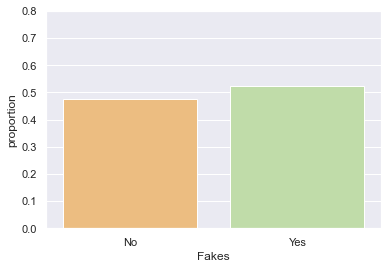
\includegraphics{output_15_1.png}
\caption{Gráfico de barras de la variable \texttt{Fake}}
\end{figure}

Las proporciones exactas de fake y no fake news son:

\begin{Shaded}
\begin{Highlighting}[]
\NormalTok{[prop\_Fake\_no , prop\_Fake\_yes]}
\end{Highlighting}
\end{Shaded}

\begin{verbatim}
[0.47701456635039424, 0.5229854336496058]
\end{verbatim}

El número exacto de fake y no fake news es:

\begin{Shaded}
\begin{Highlighting}[]
\NormalTok{[prop\_Fake\_no}\OperatorTok{*}\BuiltInTok{len}\NormalTok{(Fake\_News\_Data) , prop\_Fake\_yes}\OperatorTok{*}\BuiltInTok{len}\NormalTok{(Fake\_News\_Data)]}
\end{Highlighting}
\end{Shaded}

\begin{verbatim}
[21417.0, 23481.0]
\end{verbatim}

Eliminamos la columna \texttt{proportion\_Fakes} del data-set, que ha
sido creada solamente de manera auxiliar para poder generar el gráfico
de barras anterior:

\begin{Shaded}
\begin{Highlighting}[]
\NormalTok{Fake\_News\_Data }\OperatorTok{=}\NormalTok{ Fake\_News\_Data.loc[ : , Fake\_News\_Data.columns }\OperatorTok{!=} \StringTok{\textquotesingle{}proportion\_Fakes\textquotesingle{}}\NormalTok{]}
\end{Highlighting}
\end{Shaded}

\hypertarget{nuxfamero-de-palabras-por-noticia}{%
\subsection{Número de palabras por
noticia}\label{nuxfamero-de-palabras-por-noticia}}

Una forma de calcular en \texttt{Python} el número de palabras de cada
notica es la siguiente:

\begin{Shaded}
\begin{Highlighting}[]
\NormalTok{Fake\_News\_Data[}\StringTok{\textquotesingle{}word\_count\textquotesingle{}}\NormalTok{] }\OperatorTok{=}\NormalTok{ Fake\_News\_Data[}\StringTok{\textquotesingle{}text\textquotesingle{}}\NormalTok{].}\BuiltInTok{str}\NormalTok{.split().}\BuiltInTok{str}\NormalTok{.}\BuiltInTok{len}\NormalTok{()}
\end{Highlighting}
\end{Shaded}

Vamos a ver el data-set con la nueva columna \texttt{word\_count} que
contiene el nº de palabras por noticia

\begin{Shaded}
\begin{Highlighting}[]
\NormalTok{Fake\_News\_Data}
\end{Highlighting}
\end{Shaded}

\begin{verbatim}
      Fake   title        
      
0        1   Donald Trump Sends Out Embarrassing New Year’...   
1        1   Drunk Bragging Trump Staffer Started Russian ...   
2        1   Sheriff David Clarke Becomes An Internet Joke...   
3        1   Trump Is So Obsessed He Even Has Obama’s Name...   
4        1   Pope Francis Just Called Out Donald Trump Dur...

...    ...                                                ...   

44893    0  'Fully committed' NATO backs new U.S. approach...   
44894    0  LexisNexis withdrew two products from Chinese ...   
44895    0  Minsk cultural hub becomes haven from authorities   
44896    0  Vatican upbeat on possibility of Pope Francis ...   
44897    0  Indonesia to buy $1.14 billion worth of Russia...   



       text                                               date               
       
0      Donald Trump just couldn t wish all Americans ...  December 31, 2017   
1      House Intelligence Committee Chairman Devin Nu...  December 31, 2017   
2      On Friday, it was revealed that former Milwauk...  December 30, 2017   
3      On Christmas day, Donald Trump announced that ...  December 29, 2017   
4      Pope Francis used his annual Christmas Day mes...  December 25, 2017   

...                                                  ...                ...   

44893  BRUSSELS (Reuters) - NATO allies on Tuesday we...   August 22, 2017    
44894  LONDON (Reuters) - LexisNexis, a provider of l...   August 22, 2017    
44895  MINSK (Reuters) - In the shadow of disused Sov...   August 22, 2017    
44896  MOSCOW (Reuters) - Vatican Secretary of State ...   August 22, 2017    
44897  JAKARTA (Reuters) - Indonesia will buy 11 Sukh...   August 22, 2017    


       word_count
       
0             495  
1             305  
2             580  
3             444  
4             420  

...           ...  

44893         466  
44894         125  
44895         320  
44896         205  
44897         210  
\end{verbatim}

\hypertarget{numero-medio-de-palabras-por-noticia-en-funciuxf3n-de-si-son-fake-o-no}{%
\subsection{Numero medio de palabras por noticia en función de si son
fake o
no}\label{numero-medio-de-palabras-por-noticia-en-funciuxf3n-de-si-son-fake-o-no}}

Calculamos ahora la media de palabras de las fakes news y de la sno fake
news. Es decir, el nº medio de palabras en el cojuntos de las noticias
fake, y por otro lado en el conjutno de las no fake:

\begin{Shaded}
\begin{Highlighting}[]
\NormalTok{Fake\_News\_Data.groupby(}\StringTok{\textquotesingle{}Fake\textquotesingle{}}\NormalTok{)[}\StringTok{\textquotesingle{}word\_count\textquotesingle{}}\NormalTok{].mean()}
\end{Highlighting}
\end{Shaded}

\begin{verbatim}
Fake   Mean word_count

0        385.640099

1        423.197905
\end{verbatim}

\hypertarget{preprocesado-de-texto}{%
\section{Preprocesado de texto}\label{preprocesado-de-texto}}

En este apartado se vana a hacer una serie de operaciones orientadas al
preprocesado de texto, para poder posteriormente realizar analasis mas
profundos, y para poder implementar algoritmos de clasificación sobre
texto.

Este tipo de preprocesado es básico y fundamental en areas de la ciencia
de datos que trabajan con texto, como son la mineria de texto (text
minning), el procesamiento del lenguaje natural (PLN) y la recuperación
de información (information retrival).

Una de las operaciones centrales del preproceso de textos es la
\texttt{tokenización}.

\hypertarget{tokenizacion}{%
\subsection{Tokenizacion}\label{tokenizacion}}

Existen algunas librerias de \texttt{Python} que tienen funciones para
realizar operaciones de tokenizacion, como por ejemplo las librerias
\texttt{sklearn}, \texttt{nltk} o \texttt{spaCy}

En este caso no usaremos ninguna función de alguna de esas librerias,
sino que crearemos nuestra propia función para realizar la tokenización.

Esta función esta totalmente inspirada en la función creada por el
cientifico de datos \href{}{Joaquín Amat Rodrigo}, el cual es el creador
del excelente blog sobre ciencia de datos
\href{https://www.cienciadedatos.net/}{Cienciadedatos.net}. En este blog
Joaquin tiene un articulo sobre analisis de texto en \texttt{Python} en
el cual se encuentra la función que ahora vamos a presentar. Ademas
muchas otras partes de este trabajo estan basadas en dicho articulo, es
por ello que s ele hace una especial mención tanto aqui como en el
apartado de bibliografia.

La función \texttt{limpiar\_tokenizar} toma como input texto y devuelve
como output un vector de tokens asociado a ese texto, es decir, un
vector con las cadenas caracteres del texto, pero no con cualquier tipo,
sino que la función no considera signos de puntuación , palabras que
empiezan por ``http'', números, espacios en blancos múltiples, tokens
con longitud menor que 2.

Un token aqui es considerado como una cadena de caracteres, es decir,
una concatenacion de símbolos (sin considerar el espacio en blanco como
un símbolo).

Veamos un ejemplo de lo que consideramos tokens:

Dado el siguiente texto:

'' Esto es 1 ejemplo de l'limpieza de6 TEXTO
\url{https://t.co/rnHPgyhx4Z} @cienciadedatos \#textmining ''

Los tokens (en sentido estricto, no en el sentido restrictivo que
considera la función \texttt{limpiar\_tokenizar} ) asociados a dicho
texto son:

{[} Esto , es , 1 , ejemplo , de , l\textquotesingle limpieza , de6 ,
TEXTO , https://t.co/rnHPgyhx4Z , @cienciadedatos , \#textmining {]}

\begin{Shaded}
\begin{Highlighting}[]
\KeywordTok{def}\NormalTok{ limpiar\_tokenizar(texto):}

    \ImportTok{import}\NormalTok{ re}
    
    \CommentTok{\textquotesingle{}\textquotesingle{}\textquotesingle{}}
\CommentTok{    Esta función limpia y tokeniza el texto en palabras individuales.}
\CommentTok{    El orden en el que se va limpiando el texto no es arbitrario.}
\CommentTok{    El listado de signos de puntuación se ha obtenido de: print(string.punctuation)}
\CommentTok{    y re.escape(string.punctuation)}
\CommentTok{    \textquotesingle{}\textquotesingle{}\textquotesingle{}}
    
    \CommentTok{\# Se convierte todo el texto a minúsculas:}

\NormalTok{    nuevo\_texto }\OperatorTok{=}\NormalTok{ texto.lower()}
    
    
    \CommentTok{\# Eliminacion de paginas web (palabras que empiezan por "http"):}
    
    \CommentTok{\#\# Las cadenas de caracteres que sean enlaces a webs no serán consideradas como tokens}
    
\NormalTok{    nuevo\_texto }\OperatorTok{=}\NormalTok{ re.sub(}\StringTok{\textquotesingle{}http\textbackslash{}S+\textquotesingle{}}\NormalTok{, }\StringTok{\textquotesingle{} \textquotesingle{}}\NormalTok{, nuevo\_texto)}
    
    
    \CommentTok{\# Eliminacion de signos de puntuación:}
    
    \CommentTok{\#\# Si una cadena de caractrer contiene un signo de puntuacion estos serán eliminados y sustituidos por un   espacio en blanco. Si  por ejemplo tenemos las cadenas  \textquotesingle{}@FabioScielzo\textquotesingle{} y \textquotesingle{}Fabio@Scielzo\textquotesingle{} ,}
    \CommentTok{\#\# la funcion las transforma en  \textquotesingle{}FabioScielzo\textquotesingle{} en el primer caso  y en el par de cadenas \textquotesingle{}Fabio\textquotesingle{} , \textquotesingle{}Scielzo\textquotesingle{} en el segundo. Y si tenemos}
    \CommentTok{\#\# una cadena de signos d puntuacion   como \textquotesingle{}@\#!\textquotesingle{} la elimina directamente.}
    
\NormalTok{    regex }\OperatorTok{=} \StringTok{\textquotesingle{}[}\CharTok{\textbackslash{}\textbackslash{}}\StringTok{!}\CharTok{\textbackslash{}\textbackslash{}}\StringTok{"}\CharTok{\textbackslash{}\textbackslash{}}\StringTok{\#}\CharTok{\textbackslash{}\textbackslash{}}\StringTok{$}\CharTok{\textbackslash{}\textbackslash{}}\StringTok{\%}\CharTok{\textbackslash{}\textbackslash{}}\StringTok{\&}\CharTok{\textbackslash{}\textbackslash{}\textbackslash{}\textquotesingle{}\textbackslash{}\textbackslash{}}\StringTok{(}\CharTok{\textbackslash{}\textbackslash{}}\StringTok{)}\CharTok{\textbackslash{}\textbackslash{}}\StringTok{*}\CharTok{\textbackslash{}\textbackslash{}}\StringTok{+}\CharTok{\textbackslash{}\textbackslash{}}\StringTok{,}\CharTok{\textbackslash{}\textbackslash{}}\StringTok{{-}}\CharTok{\textbackslash{}\textbackslash{}}\StringTok{.}\CharTok{\textbackslash{}\textbackslash{}}\StringTok{/}\CharTok{\textbackslash{}\textbackslash{}}\StringTok{:}\CharTok{\textbackslash{}\textbackslash{}}\StringTok{;}\CharTok{\textbackslash{}\textbackslash{}}\StringTok{\textless{}}\CharTok{\textbackslash{}\textbackslash{}}\StringTok{=}\CharTok{\textbackslash{}\textbackslash{}}\StringTok{\textgreater{}}\CharTok{\textbackslash{}\textbackslash{}}\StringTok{?}\CharTok{\textbackslash{}\textbackslash{}}\StringTok{@}\CharTok{\textbackslash{}\textbackslash{}}\StringTok{[}\CharTok{\textbackslash{}\textbackslash{}\textbackslash{}\textbackslash{}\textbackslash{}\textbackslash{}}\StringTok{]}\CharTok{\textbackslash{}\textbackslash{}}\StringTok{\^{}\_}\CharTok{\textbackslash{}\textbackslash{}}\StringTok{\textasciigrave{}}\CharTok{\textbackslash{}\textbackslash{}}\StringTok{\{}\CharTok{\textbackslash{}\textbackslash{}}\StringTok{|}\CharTok{\textbackslash{}\textbackslash{}}\StringTok{\}}\CharTok{\textbackslash{}\textbackslash{}}\StringTok{\textasciitilde{}]\textquotesingle{}}
    
\NormalTok{    nuevo\_texto }\OperatorTok{=}\NormalTok{ re.sub(regex , }\StringTok{\textquotesingle{} \textquotesingle{}}\NormalTok{, nuevo\_texto)}
    
    
    \CommentTok{\# Eliminacion de numeros:}
    
    \CommentTok{\#\# Si una cadena de caracter tiene numeros estos serán eliminados y sustituidos por un espacio en blanco. Si por ejemplo tenemos las cadenas \textquotesingle{}4FabioScielzo\textquotesingle{} y \textquotesingle{}Fabio44Scielzo\textquotesingle{} la funcion las transforma en \textquotesingle{}FabioScielzo\textquotesingle{} y \textquotesingle{}Fabio\textquotesingle{} , \textquotesingle{}Scielzo\textquotesingle{} , respectivamente. Ademas si una cadena solo contienen numeros, por ejemplo \textquotesingle{}123\textquotesingle{} la elimina directamente.}
    
\NormalTok{    nuevo\_texto }\OperatorTok{=}\NormalTok{ re.sub(}\StringTok{"\textbackslash{}d+"}\NormalTok{, }\StringTok{\textquotesingle{} \textquotesingle{}}\NormalTok{, nuevo\_texto)}
    
    
    
    \CommentTok{\# Eliminacion de espacios en blanco multiples:}
    
    \CommentTok{\#\# Si tenemos en un texto dos o mas espacios en blanco consecutivos la funcion los transforma en un solo espacio en blanco. Por ejemplo si tenemos el texto "Fabio     es abogado" la funcion lo transforma en "Fabio es abogado".}
    
\NormalTok{    nuevo\_texto }\OperatorTok{=}\NormalTok{ re.sub(}\StringTok{"}\CharTok{\textbackslash{}\textbackslash{}}\StringTok{s+"}\NormalTok{, }\StringTok{\textquotesingle{} \textquotesingle{}}\NormalTok{, nuevo\_texto)}
    
    
    \CommentTok{\# Una vez que a un texto se le han aplicado las operaciones anteriores ya solo quede considerar las cadenas de caracteres de ese texto como tokens, ya que son cadenas con buenas propiedades, a saber, sin signos de puntuacion, sin numeros, sin links de web. Ademas la eliminacion de espacios en blanco multiples es fundamental para que la siguiente operacion funcione bien, ya que en el texto final resultante todas las cadenas estan separadas entre si por un solo espacio, y la siguiente operacion utiliza esa propiedad para identificar a las cadenas, que ya serán considerados tokens en sentido estricto.}
    
    \CommentTok{\# Obtención de tokens:}
    
\NormalTok{    nuevo\_texto }\OperatorTok{=}\NormalTok{ nuevo\_texto.split(sep }\OperatorTok{=} \StringTok{\textquotesingle{} \textquotesingle{}}\NormalTok{)}
    
    
    \CommentTok{\# Eliminacion de tokens con una longitud menor que  2:}
    
    \CommentTok{\#\# Una ultima operacion es solo considerar los tokens obteenidos tras las operaciones anteriores que tengan un tamaño (nº de caracteres) igual o superior a 2 , es decir, dejar fuera tokens con solo un caracter.}
    
\NormalTok{    nuevo\_texto }\OperatorTok{=}\NormalTok{ [token }\ControlFlowTok{for}\NormalTok{ token }\KeywordTok{in}\NormalTok{ nuevo\_texto }\ControlFlowTok{if} \BuiltInTok{len}\NormalTok{(token) }\OperatorTok{\textgreater{}=}  \DecValTok{2}\NormalTok{]}
    
    \ControlFlowTok{return}\NormalTok{(nuevo\_texto)}
\end{Highlighting}
\end{Shaded}

Probamos el funcionamiento de la función \texttt{limpiar\_tokenizar} con
el mismo texto que fue usado antes como ejemplo ilustrativo.

\begin{Shaded}
\begin{Highlighting}[]

\NormalTok{test }\OperatorTok{=} \StringTok{"Esto es 1 ejemplo de l\textquotesingle{}limpieza de6 TEXTO  https://t.co/rnHPgyhx4Z @cienciadedatos \#textmining"}

\BuiltInTok{print}\NormalTok{(limpiar\_tokenizar(texto}\OperatorTok{=}\NormalTok{test))}
\end{Highlighting}
\end{Shaded}

\begin{verbatim}
['esto', 'es', 'ejemplo', 'de', 'limpieza', 'de', 'texto', 'cienciadedatos', 'textmining']
\end{verbatim}

Ahora probamos la función \texttt{limpiar\_tokenizar} con la primera
noticia del data-set \texttt{Fake\_News\_Data}:

\begin{Shaded}
\begin{Highlighting}[]
\NormalTok{Fake\_News\_Data[}\StringTok{\textquotesingle{}text\textquotesingle{}}\NormalTok{][}\DecValTok{0}\NormalTok{]}
\end{Highlighting}
\end{Shaded}

\begin{verbatim}
'Donald Trump just couldn t wish all Americans a Happy New Year and leave it at that. Instead, he had to give a shout out to his enemies, haters and  the very dishonest fake news media.  The former reality show star had just one job to do and he couldn t do it. As our Country rapidly grows stronger and smarter, I want to wish all of my friends, supporters, enemies, haters, and even the very dishonest Fake News Media, a Happy and Healthy New Year,  President Angry Pants tweeted.  2018 will be a great year for America! As our Country rapidly grows stronger and smarter, I want to wish all of my friends, supporters, enemies, haters, and even the very dishonest Fake News Media, a Happy and Healthy New Year. 2018 will be a great year for America!  Donald J. Trump (@realDonaldTrump) December 31, 2017Trump s tweet went down about as welll as you d expect.What kind of president sends a New Year s greeting like this despicable, petty, infantile gibberish? Only Trump! His lack of decency won t even allow him to rise above the gutter long enough to wish the American citizens a happy new year!  Bishop Talbert Swan (@TalbertSwan) December 31, 2017no one likes you  Calvin (@calvinstowell) December 31, 2017Your impeachment would make 2018 a great year for America, but I ll also accept regaining control of Congress.  Miranda Yaver (@mirandayaver) December 31, 2017Do you hear yourself talk? When you have to include that many people that hate you you have to wonder? Why do the they all hate me?  Alan Sandoval (@AlanSandoval13) December 31, 2017Who uses the word Haters in a New Years wish??  Marlene (@marlene399) December 31, 2017You can t just say happy new year?  Koren pollitt (@Korencarpenter) December 31, 2017Here s Trump s New Year s Eve tweet from 2016.Happy New Year to all, including to my many enemies and those who have fought me and lost so badly they just don t know what to do. Love!  Donald J. Trump (@realDonaldTrump) December 31, 2016This is nothing new for Trump. He s been doing this for years.Trump has directed messages to his  enemies  and  haters  for New Year s, Easter, Thanksgiving, and the anniversary of 9/11. pic.twitter.com/4FPAe2KypA  Daniel Dale (@ddale8) December 31, 2017Trump s holiday tweets are clearly not presidential.How long did he work at Hallmark before becoming President?  Steven Goodine (@SGoodine) December 31, 2017He s always been like this . . . the only difference is that in the last few years, his filter has been breaking down.  Roy Schulze (@thbthttt) December 31, 2017Who, apart from a teenager uses the term haters?  Wendy (@WendyWhistles) December 31, 2017he s a fucking 5 year old  Who Knows (@rainyday80) December 31, 2017So, to all the people who voted for this a hole thinking he would change once he got into power, you were wrong! 70-year-old men don t change and now he s a year older.Photo by Andrew Burton/Getty Images.'
\end{verbatim}

\begin{Shaded}
\begin{Highlighting}[]
\BuiltInTok{print}\NormalTok{(limpiar\_tokenizar(texto}\OperatorTok{=}\NormalTok{Fake\_News\_Data[}\StringTok{\textquotesingle{}text\textquotesingle{}}\NormalTok{][}\DecValTok{0}\NormalTok{]))}
\end{Highlighting}
\end{Shaded}

\begin{verbatim}
['donald', 'trump', 'just', 'couldn', 'wish', 'all', 'americans', 'happy', 'new', 'year', 'and', 'leave', 'it', 'at', 'that', 'instead', 'he', 'had', 'to', 'give', 'shout', 'out', 'to', 'his', 'enemies', 'haters', 'and', 'the', 'very', 'dishonest', 'fake', 'news', 'media', 'the', 'former', 'reality', 'show', 'star', 'had', 'just', 'one', 'job', 'to', 'do', 'and', 'he', 'couldn', 'do', 'it', 'as', 'our', 'country', 'rapidly', 'grows', 'stronger', 'and', 'smarter', 'want', 'to', 'wish', 'all', 'of', 'my', 'friends', 'supporters', 'enemies', 'haters', 'and', 'even', 'the', 'very', 'dishonest', 'fake', 'news', 'media', 'happy', 'and', 'healthy', 'new', 'year', 'president', 'angry', 'pants', 'tweeted', 'will', 'be', 'great', 'year', 'for', 'america', 'as', 'our', 'country', 'rapidly', 'grows', 'stronger', 'and', 'smarter', 'want', 'to', 'wish', 'all', 'of', 'my', 'friends', 'supporters', 'enemies', 'haters', 'and', 'even', 'the', 'very', 'dishonest', 'fake', 'news', 'media', 'happy', 'and', 'healthy', 'new', 'year', 'will', 'be', 'great', 'year', 'for', 'america', 'donald', 'trump', 'realdonaldtrump', 'december', 'trump', 'tweet', 'went', 'down', 'about', 'as', 'welll', 'as', 'you', 'expect', 'what', 'kind', 'of', 'president', 'sends', 'new', 'year', 'greeting', 'like', 'this', 'despicable', 'petty', 'infantile', 'gibberish', 'only', 'trump', 'his', 'lack', 'of', 'decency', 'won', 'even', 'allow', 'him', 'to', 'rise', 'above', 'the', 'gutter', 'long', 'enough', 'to', 'wish', 'the', 'american', 'citizens', 'happy', 'new', 'year', 'bishop', 'talbert', 'swan', 'talbertswan', 'december', 'no', 'one', 'likes', 'you', 'calvin', 'calvinstowell', 'december', 'your', 'impeachment', 'would', 'make', 'great', 'year', 'for', 'america', 'but', 'll', 'also', 'accept', 'regaining', 'control', 'of', 'congress', 'miranda', 'yaver', 'mirandayaver', 'december', 'do', 'you', 'hear', 'yourself', 'talk', 'when', 'you', 'have', 'to', 'include', 'that', 'many', 'people', 'that', 'hate', 'you', 'you', 'have', 'to', 'wonder', 'why', 'do', 'the', 'they', 'all', 'hate', 'me', 'alan', 'sandoval', 'alansandoval', 'december', 'who', 'uses', 'the', 'word', 'haters', 'in', 'new', 'years', 'wish', 'marlene', 'marlene', 'december', 'you', 'can', 'just', 'say', 'happy', 'new', 'year', 'koren', 'pollitt', 'korencarpenter', 'december', 'here', 'trump', 'new', 'year', 'eve', 'tweet', 'from', 'happy', 'new', 'year', 'to', 'all', 'including', 'to', 'my', 'many', 'enemies', 'and', 'those', 'who', 'have', 'fought', 'me', 'and', 'lost', 'so', 'badly', 'they', 'just', 'don', 'know', 'what', 'to', 'do', 'love', 'donald', 'trump', 'realdonaldtrump', 'december', 'this', 'is', 'nothing', 'new', 'for', 'trump', 'he', 'been', 'doing', 'this', 'for', 'years', 'trump', 'has', 'directed', 'messages', 'to', 'his', 'enemies', 'and', 'haters', 'for', 'new', 'year', 'easter', 'thanksgiving', 'and', 'the', 'anniversary', 'of', 'pic', 'twitter', 'com', 'fpae', 'kypa', 'daniel', 'dale', 'ddale', 'december', 'trump', 'holiday', 'tweets', 'are', 'clearly', 'not', 'presidential', 'how', 'long', 'did', 'he', 'work', 'at', 'hallmark', 'before', 'becoming', 'president', 'steven', 'goodine', 'sgoodine', 'december', 'he', 'always', 'been', 'like', 'this', 'the', 'only', 'difference', 'is', 'that', 'in', 'the', 'last', 'few', 'years', 'his', 'filter', 'has', 'been', 'breaking', 'down', 'roy', 'schulze', 'thbthttt', 'december', 'who', 'apart', 'from', 'teenager', 'uses', 'the', 'term', 'haters', 'wendy', 'wendywhistles', 'december', 'he', 'fucking', 'year', 'old', 'who', 'knows', 'rainyday', 'december', 'so', 'to', 'all', 'the', 'people', 'who', 'voted', 'for', 'this', 'hole', 'thinking', 'he', 'would', 'change', 'once', 'he', 'got', 'into', 'power', 'you', 'were', 'wrong', 'year', 'old', 'men', 'don', 'change', 'and', 'now', 'he', 'year', 'older', 'photo', 'by', 'andrew', 'burton', 'getty', 'images']
\end{verbatim}

Ahora aplicamos la función \texttt{limpiar\_tokenizar} a cada una de las
noticias del data-set \texttt{Fake\_News\_Data}

\begin{Shaded}
\begin{Highlighting}[]
\NormalTok{Fake\_News\_Data[}\StringTok{\textquotesingle{}text\_tokenizado\textquotesingle{}}\NormalTok{] }\OperatorTok{=}\NormalTok{ Fake\_News\_Data[}\StringTok{\textquotesingle{}text\textquotesingle{}}\NormalTok{].}\BuiltInTok{apply}\NormalTok{( limpiar\_tokenizar )}
\end{Highlighting}
\end{Shaded}

Creamos una columna que identifique las noticias:

\begin{Shaded}
\begin{Highlighting}[]
\NormalTok{Fake\_News\_Data[}\StringTok{\textquotesingle{}id\_text\textquotesingle{}}\NormalTok{] }\OperatorTok{=} \BuiltInTok{range}\NormalTok{(}\DecValTok{0}\NormalTok{, }\BuiltInTok{len}\NormalTok{(Fake\_News\_Data))}
\end{Highlighting}
\end{Shaded}

Vemos como queda tras estos cambios el data-set
\texttt{Fake\_News\_Data}:

\begin{Shaded}
\begin{Highlighting}[]
\NormalTok{Fake\_News\_Data}
\end{Highlighting}
\end{Shaded}

\begin{verbatim}
      Fake                    title                                            
      
0        1   Donald Trump Sends Out Embarrassing New Year’...   
1        1   Drunk Bragging Trump Staffer Started Russian ...   
2        1   Sheriff David Clarke Becomes An Internet Joke...   
3        1   Trump Is So Obsessed He Even Has Obama’s Name...   
4        1   Pope Francis Just Called Out Donald Trump Dur...   

...    ...                     ...   

44893    0  'Fully committed' NATO backs new U.S. approach...   
44894    0  LexisNexis withdrew two products from Chinese ...   
44895    0  Minsk cultural hub becomes haven from authorities   
44896    0  Vatican upbeat on possibility of Pope Francis ...   
44897    0  Indonesia to buy $1.14 billion worth of Russia...   


                         text                                   date                

0      Donald Trump just couldn t wish all Americans ...  December 31, 2017   
1      House Intelligence Committee Chairman Devin Nu...  December 31, 2017   
2      On Friday, it was revealed that former Milwauk...  December 30, 2017   
3      On Christmas day, Donald Trump announced that ...  December 29, 2017   
4      Pope Francis used his annual Christmas Day mes...  December 25, 2017 

...                     ...                                      ...   

44893  BRUSSELS (Reuters) - NATO allies on Tuesday we...   August 22, 2017    
44894  LONDON (Reuters) - LexisNexis, a provider of l...   August 22, 2017    
44895  MINSK (Reuters) - In the shadow of disused Sov...   August 22, 2017    
44896  MOSCOW (Reuters) - Vatican Secretary of State ...   August 22, 2017    
44897  JAKARTA (Reuters) - Indonesia will buy 11 Sukh...   August 22, 2017   


       word_count              text_tokenizado                        id_text  

0         495     [donald, trump, just, couldn, wish, all, ameri...      0  
1         305     [house, intelligence, committee, chairman, dev...      1  
2         580     [on, friday, it, was, revealed, that, former, ...      2  
3         444     [on, christmas, day, donald, trump, announced,...      3  
4         420     [pope, francis, used, his, annual, christmas, ...      4  

...       ...                        ...                                ...  

44893     466     [brussels, reuters, nato, allies, on, tuesday,...    44893  
44894     125     [london, reuters, lexisnexis, provider, of, le...    44894  
44895     320     [minsk, reuters, in, the, shadow, of, disused,...    44895  
44896     205     [moscow, reuters, vatican, secretary, of, stat...    44896  
44897     210     [jakarta, reuters, indonesia, will, buy, sukho...    44897  
\end{verbatim}

Creamos un nuevo data-frame solo con las columnas (variables)
\texttt{id\_text} , \texttt{text\_tokenizado} y \texttt{Fake}, en ell
que la columna \texttt{text\_tokenizado} esta expandida, es decir, al
ser una columna cuyos elementos son vectores, lo que se hace con la
operacion \texttt{explode} es expandir cada uno de esos vectores en un
nuevo data-frame, es decir, para cada uno de esos vectores se crean
tantas filas en el nuevo data-frame como elementos hay en el vector, y
en cada una de esas filas la columna \texttt{text\_tokenizado} contendra
un elemento del vector expandido. Visualmente es mas facil de entenderlo
como se verá a continuación:

\begin{Shaded}
\begin{Highlighting}[]
\NormalTok{Fake\_News\_Tokens }\OperatorTok{=}\NormalTok{ Fake\_News\_Data.loc[:, [}\StringTok{\textquotesingle{}id\_text\textquotesingle{}}\NormalTok{, }\StringTok{\textquotesingle{}text\_tokenizado\textquotesingle{}}\NormalTok{, }\StringTok{\textquotesingle{}Fake\textquotesingle{}}\NormalTok{] ].explode(column}\OperatorTok{=}\StringTok{\textquotesingle{}text\_tokenizado\textquotesingle{}}\NormalTok{)}


\CommentTok{\# Renombramos la columna \textasciigrave{}text\_tokenizado\textasciigrave{} como \textasciigrave{}token\textasciigrave{} :}

\NormalTok{Fake\_News\_Tokens }\OperatorTok{=}\NormalTok{ Fake\_News\_Tokens.rename(columns}\OperatorTok{=}\NormalTok{\{}\StringTok{\textquotesingle{}text\_tokenizado\textquotesingle{}}\NormalTok{:}\StringTok{\textquotesingle{}token\textquotesingle{}}\NormalTok{\})}
\end{Highlighting}
\end{Shaded}

Imprimimos el nuevo data-frame creado \texttt{Fake\_News\_Tokens} al
expandir la columna \texttt{text\_tokenizado} del data-frame
\texttt{Fake\_News\_Data}

\begin{Shaded}
\begin{Highlighting}[]
\NormalTok{Fake\_News\_Tokens}
\end{Highlighting}
\end{Shaded}

\begin{verbatim}
       id_text       token    Fake
0            0      donald      1
0            0       trump      1
0            0        just      1
0            0      couldn      1
0            0        wish      1

...        ...         ...     ...

44897    44897  technology      0
44897    44897         and      0
44897    44897    aviation      0
44897    44897       among      0
44897    44897      others      0
\end{verbatim}

\newpage

\hypertarget{descripciuxf3n-estaduxedstica-de-los-datos-tras-la-tokenizaciuxf3n}{%
\section{\texorpdfstring{Descripción estadística de los datos tras la
\texttt{tokenización}}{Descripción estadística de los datos tras la tokenización}}\label{descripciuxf3n-estaduxedstica-de-los-datos-tras-la-tokenizaciuxf3n}}

\hypertarget{numero-de-tokens-del-conjunto-de-noticias-en-funcion-de-si-son-fake-o-no}{%
\subsection{Numero de tokens del conjunto de noticias en funcion de si
son fake o
no}\label{numero-de-tokens-del-conjunto-de-noticias-en-funcion-de-si-son-fake-o-no}}

\begin{Shaded}
\begin{Highlighting}[]
\CommentTok{\# nº de palabras (tokens) en el conjunto de textos clasificados como fake y en los no fake}

\NormalTok{Fake\_News\_Tokens.groupby(by}\OperatorTok{=}\StringTok{\textquotesingle{}Fake\textquotesingle{}}\NormalTok{)[}\StringTok{\textquotesingle{}token\textquotesingle{}}\NormalTok{].count()}
\end{Highlighting}
\end{Shaded}

\begin{verbatim}
Fake
0    7891501
1    9611544
Name: token, dtype: int64
\end{verbatim}

\hypertarget{numero-de-tokens-uxfanicos-del-conjunto-de-noticias-en-funcion-de-si-son-fake-o-no}{%
\subsection{\texorpdfstring{Numero de tokens \emph{únicos} del conjunto
de noticias en funcion de si son fake o
no}{Numero de tokens únicos del conjunto de noticias en funcion de si son fake o no}}\label{numero-de-tokens-uxfanicos-del-conjunto-de-noticias-en-funcion-de-si-son-fake-o-no}}

\begin{Shaded}
\begin{Highlighting}[]
\CommentTok{\# nº de palabras (tokens) *unicos* en el conjunto de textos clasificados como fake y en los no fake}

\NormalTok{Fake\_News\_Tokens.groupby(by}\OperatorTok{=}\StringTok{\textquotesingle{}Fake\textquotesingle{}}\NormalTok{)[}\StringTok{\textquotesingle{}token\textquotesingle{}}\NormalTok{].nunique()}
\end{Highlighting}
\end{Shaded}

\begin{verbatim}
Fake
0    78020
1    85642
Name: token, dtype: int64
\end{verbatim}

\hypertarget{numero-de-tokens-en-cada-una-de-las-noticias-individualmente}{%
\subsection{Numero de tokens en cada una de las noticias
individualmente}\label{numero-de-tokens-en-cada-una-de-las-noticias-individualmente}}

\begin{Shaded}
\begin{Highlighting}[]
\CommentTok{\# nº de palabras (tokens) en cada texto individual clasificados como fake y en los no fake}

\NormalTok{df1 }\OperatorTok{=}\NormalTok{ pd.DataFrame( Fake\_News\_Tokens.groupby(by }\OperatorTok{=}\NormalTok{ [}\StringTok{"id\_text"}\NormalTok{ , }\StringTok{"Fake"}\NormalTok{] )[}\StringTok{"token"}\NormalTok{].count().rename(}\StringTok{\textquotesingle{}nº\_tokens\textquotesingle{}}\NormalTok{) )}
\end{Highlighting}
\end{Shaded}

\begin{Shaded}
\begin{Highlighting}[]
\NormalTok{df1}
\end{Highlighting}
\end{Shaded}

\begin{verbatim}
                     nº_tokens
id_text   Fake           
  0         1           447
  1         1           294
  2         1           563
  3         1           426
  4         1           415

 ...       ...          ...

44893       0           433
44894       0           120
44895       0           307
44896       0           196
44897       0           197
\end{verbatim}

Hay noticias que no tienen tokens :

\begin{Shaded}
\begin{Highlighting}[]
\NormalTok{df1.loc[df1[}\StringTok{\textquotesingle{}nº\_tokens\textquotesingle{}}\NormalTok{] }\OperatorTok{==} \DecValTok{0}\NormalTok{, :]}
\end{Highlighting}
\end{Shaded}

\begin{verbatim}
                 nº_tokens
id_text  Fake           

9358      1           0
10923     1           0
11041     1           0
11190     1           0
11225     1           0

 ...     ...         ...

21857     1           0
21869     1           0
21870     1           0
21873     1           0
32451     0           0
\end{verbatim}

Algunos ejemplos de estas noticias son los siguientes:

\begin{Shaded}
\begin{Highlighting}[]
\NormalTok{Fake\_News\_Data.loc[Fake\_News\_Data.id\_text }\OperatorTok{==} \DecValTok{9358}\NormalTok{]}
\end{Highlighting}
\end{Shaded}

\begin{verbatim}
        Fake   title  
9358     1     https://100percentfedup.com/served-roy-moore-v...   


        text  
9358    https://100percentfedup.com/served-roy-moore-v...   


        date  word_count  
9358              1   


      text_tokenizado   id_text  
9358        []           9358  
\end{verbatim}

\begin{Shaded}
\begin{Highlighting}[]
\NormalTok{Fake\_News\_Data.loc[Fake\_News\_Data.id\_text }\OperatorTok{==} \DecValTok{10923}\NormalTok{]}
\end{Highlighting}
\end{Shaded}

\begin{verbatim}
       Fake      title 
10923    1       TAKE OUR POLL: Who Do You Think President Trum...        

       text     date            word_count   text_tokenizado   id_text  
10923           May 10, 2017        0              []           10923
\end{verbatim}

Nos quedamos por tanto solo con las noticias que tienen algun token :

\begin{Shaded}
\begin{Highlighting}[]
\NormalTok{df2 }\OperatorTok{=}\NormalTok{ df1.loc[df1[}\StringTok{\textquotesingle{}nº\_tokens\textquotesingle{}}\NormalTok{] }\OperatorTok{!=} \DecValTok{0}\NormalTok{, :]}

\NormalTok{df2}
\end{Highlighting}
\end{Shaded}

\begin{verbatim}
                 nº_tokens
id_text   Fake           

0          1           447
1          1           294
2          1           563
3          1           426
4          1           415

...       ...          ...

44893      0           433
44894      0           120
44895      0           307
44896      0           196
44897      0           197
\end{verbatim}

Calculamos el numero medio de tokens para las noticas que tienen uno o
mas tokens en funcion se si son fake o no:

\begin{Shaded}
\begin{Highlighting}[]
\NormalTok{df2.groupby(}\StringTok{"Fake"}\NormalTok{)[}\StringTok{"nº\_tokens"}\NormalTok{].agg([}\StringTok{\textquotesingle{}mean\textquotesingle{}}\NormalTok{])}
\end{Highlighting}
\end{Shaded}

\begin{verbatim}
            mean
Fake            
0     368.486225
1     422.169983
\end{verbatim}

Se puede interpretar como la longitud media de las noticas fake y de las
no fake

\vspace{0.5cm}

Hay diferencias entre lo obtenido mediante esta operación y lo obtenido
al usar el siguiente código, que fue visto anteriormente:

\begin{Shaded}
\begin{Highlighting}[]
\NormalTok{Fake\_News\_Data[}\StringTok{\textquotesingle{}word\_count\textquotesingle{}}\NormalTok{] }\OperatorTok{=}\NormalTok{ Fake\_News\_Data[}\StringTok{\textquotesingle{}text\textquotesingle{}}\NormalTok{].}\BuiltInTok{str}\NormalTok{.split().}\BuiltInTok{str}\NormalTok{.}\BuiltInTok{len}\NormalTok{()}

\NormalTok{Fake\_News\_Data.groupby(}\StringTok{\textquotesingle{}Fake\textquotesingle{}}\NormalTok{)[}\StringTok{\textquotesingle{}word\_count\textquotesingle{}}\NormalTok{].mean()}
\end{Highlighting}
\end{Shaded}

\begin{verbatim}
Fake   Mean word_count
    
0        385.640099
    
1        423.197905
\end{verbatim}

Y esto es debido a que el código
\texttt{Fake\_News\_Data{[}\textquotesingle{}text\textquotesingle{}{]}.str.split()}
hace una operacion similar a la realizada por nuestra funcion
\texttt{limpiar\_tokenizar} pero \textbf{no exactamente igual}, y esto
lleva a que con la primera opcion se obtiene un conjunto de tokens
diferente al obtenido con la funcion \texttt{limpiar\_tokenizar}, en los
distintos documentos, y esto lleva a que la longitud de los documentos
sea diferente si se consideran los tokens obtenidos con
\texttt{Fake\_News\_Data{[}\textquotesingle{}text\textquotesingle{}{]}.str.split()}
a si se usan los obtenidos con \texttt{limpiar\_tokenizar}, llo que
lleva a diferencias en las longitudes medias obtenidas.

\begin{Shaded}
\begin{Highlighting}[]
\NormalTok{Fake\_News\_Data[}\StringTok{\textquotesingle{}text\textquotesingle{}}\NormalTok{].}\BuiltInTok{str}\NormalTok{.split()}
\end{Highlighting}
\end{Shaded}

\begin{verbatim}

0        [Donald, Trump, just, couldn, t, wish, all, Am...
1        [House, Intelligence, Committee, Chairman, Dev...
2        [On, Friday,, it, was, revealed, that, former,...
3        [On, Christmas, day,, Donald, Trump, announced...
4        [Pope, Francis, used, his, annual, Christmas, ...
                               ...                        
44893    [BRUSSELS, (Reuters), -, NATO, allies, on, Tue...
44894    [LONDON, (Reuters), -, LexisNexis,, a, provide...
44895    [MINSK, (Reuters), -, In, the, shadow, of, dis...
44896    [MOSCOW, (Reuters), -, Vatican, Secretary, of,...
44897    [JAKARTA, (Reuters), -, Indonesia, will, buy, ...
\end{verbatim}

Como se pueden ver con el código anterior se obtiene por ejemplo que `-'
y `, Donald' son tokens , cuando con la función
\texttt{limpiar\_tokenizar} no serían considerados un tokens.

\vspace{0.5cm}

Otra forma de calcular lo anterior:

\begin{Shaded}
\begin{Highlighting}[]
\NormalTok{m0 }\OperatorTok{=}\NormalTok{ ( Fake\_News\_Tokens.loc[Fake\_News\_Tokens[}\StringTok{\textquotesingle{}Fake\textquotesingle{}}\NormalTok{]}\OperatorTok{==}\DecValTok{0}\NormalTok{].groupby(}\StringTok{\textquotesingle{}id\_text\textquotesingle{}}\NormalTok{)[}\StringTok{\textquotesingle{}token\textquotesingle{}}\NormalTok{].count() ).mean()}
\end{Highlighting}
\end{Shaded}

\begin{Shaded}
\begin{Highlighting}[]
\NormalTok{m1 }\OperatorTok{=}\NormalTok{ ( Fake\_News\_Tokens.loc[Fake\_News\_Tokens[}\StringTok{\textquotesingle{}Fake\textquotesingle{}}\NormalTok{]}\OperatorTok{==}\DecValTok{1}\NormalTok{].groupby(}\StringTok{\textquotesingle{}id\_text\textquotesingle{}}\NormalTok{)[}\StringTok{\textquotesingle{}token\textquotesingle{}}\NormalTok{].count() ).mean()}
\end{Highlighting}
\end{Shaded}

\begin{Shaded}
\begin{Highlighting}[]
\NormalTok{pd.DataFrame(\{}\StringTok{\textquotesingle{}fake\_new\textquotesingle{}}\NormalTok{: [}\DecValTok{0}\NormalTok{,}\DecValTok{1}\NormalTok{] , }\StringTok{\textquotesingle{}tokens\_mean\textquotesingle{}}\NormalTok{:[m0 , m1]\})}
\end{Highlighting}
\end{Shaded}

\begin{verbatim}
   fake_new  tokens_mean
0         0   368.469020
1         1   409.332822
\end{verbatim}

\hypertarget{nuxfamero-de-veces-que-aparece-cada-token-en-el-conjunto-de-las-noticias-en-funcion-de-si-es-fake-o-no}{%
\subsection{Número de veces que aparece cada token en el conjunto de las
noticias en funcion de si es fake o
no}\label{nuxfamero-de-veces-que-aparece-cada-token-en-el-conjunto-de-las-noticias-en-funcion-de-si-es-fake-o-no}}

\begin{Shaded}
\begin{Highlighting}[]
\NormalTok{df }\OperatorTok{=}\NormalTok{ pd.DataFrame(  (Fake\_News\_Tokens.groupby(by }\OperatorTok{=}\NormalTok{ [}\StringTok{"Fake"}\NormalTok{, }\StringTok{"token"}\NormalTok{] )[}\StringTok{"token"}\NormalTok{].count().unstack(fill\_value}\OperatorTok{=}\DecValTok{0}\NormalTok{).stack().reset\_index(name}\OperatorTok{=}\StringTok{\textquotesingle{}frecuencia\_token\textquotesingle{}}\NormalTok{)))}

\CommentTok{\# .unstack(fill\_value=0).stack() para que tambien aparezcan los tokens con count = 0 , si no solo aprecerian los que tienen count \textgreater{} 0.}

\NormalTok{df}
\end{Highlighting}
\end{Shaded}

\begin{verbatim}
        Fake       token  frecuencia_token
0          0          aa                22
1          0         aaa                 7
2          0  aaaaaaaand                 0
3          0   aaaaackkk                 0
4          0  aaaaapkfhk                 0

...      ...         ...               ...

251605     1        ””it                 0
251606     1      ””when                 0
251607     1         •if                 0
251608     1      $emoji1$               0
251609     1      $emoji2$               0
\end{verbatim}

La salida anterior nos da para cada token el numero de veces que aparece
en el conjunto de las fake news por un lado (Fake = 1), y por otro lado
en el conjunto de las no fake (Fake=0)

Veamos algunos ejemplos para tokens concretos:

En la siguiente salida vemos el nº de veces que aparece el token `yes'
en eñ conjunto de las fake news (1775), asi como en el conjunto de las
no fake news (336).

\begin{Shaded}
\begin{Highlighting}[]
\NormalTok{df.loc[df[}\StringTok{\textquotesingle{}token\textquotesingle{}}\NormalTok{]}\OperatorTok{==}\StringTok{\textquotesingle{}yes\textquotesingle{}}\NormalTok{ , ] }\CommentTok{\# El token \textquotesingle{}yes\textquotesingle{} aprece 1775 veces en el conjunto de las fake news y 336 en el de las no fake news}
\end{Highlighting}
\end{Shaded}

\begin{verbatim}
        Fake token  frecuencia_token
116577     0   yes               336
242382     1   yes              1775
\end{verbatim}

En la siguiente salida vemos el nº de veces que aparece el token `true'
en eñ conjunto de las fake news (2595), asi como en el conjunto de las
no fake news (412).

\begin{Shaded}
\begin{Highlighting}[]
\NormalTok{df.loc[df[}\StringTok{\textquotesingle{}token\textquotesingle{}}\NormalTok{]}\OperatorTok{==}\StringTok{\textquotesingle{}true\textquotesingle{}}\NormalTok{ , ] }\CommentTok{\# El token \textquotesingle{}true\textquotesingle{} aparece 2595 veces en el conjunto de las fake news y 412 en el de las no fake news}
\end{Highlighting}
\end{Shaded}

\begin{verbatim}
        Fake token  frecuencia_token
106608     0  true               412
232413     1  true              2595
\end{verbatim}

En la siguiente salida podemos ver el nº de veces que aparece cada token
en el conjunto de las no fake news.

\begin{Shaded}
\begin{Highlighting}[]
\NormalTok{df.loc[df[}\StringTok{\textquotesingle{}Fake\textquotesingle{}}\NormalTok{]}\OperatorTok{==}\DecValTok{0}\NormalTok{ , ] }
\end{Highlighting}
\end{Shaded}

\begin{verbatim}
         Fake       token  frecuencia_token
         
0          0          aa                22
1          0         aaa                 7
2          0  aaaaaaaand                 0
3          0   aaaaackkk                 0
4          0  aaaaapkfhk                 0

...      ...         ...               ...

125800     0        ””it                 1
125801     0      ””when                 1
125802     0         •if                 3
125803     0      $emoji1$               3
125804     0      $emoji2$               1
\end{verbatim}

Y en la siguiente salida podemos ver el nº de veces que aparece cada
token en el conjunto de las fake news.

\begin{Shaded}
\begin{Highlighting}[]
\NormalTok{df.loc[df[}\StringTok{\textquotesingle{}Fake\textquotesingle{}}\NormalTok{]}\OperatorTok{==}\DecValTok{1}\NormalTok{ , ] }
\end{Highlighting}
\end{Shaded}

\begin{verbatim}
        Fake       token  frecuencia_token
125805     1          aa                24
125806     1         aaa                 9
125807     1  aaaaaaaand                 1
125808     1   aaaaackkk                 1
125809     1  aaaaapkfhk                 1
...      ...         ...               ...
251605     1        ””it                 0
251606     1      ””when                 0
251607     1         •if                 0
251608     1      $emoji1$               0
251609     1      $emoji2$               0
\end{verbatim}

\hypertarget{ranking-de-tokens-mas-frecuentes-en-el-conjunto-de-las-noticas-en-funcion-de-si-son-fake-y-no-fake}{%
\subsection{Ranking de tokens mas frecuentes en el conjunto de las
noticas en funcion de si son fake y no
fake}\label{ranking-de-tokens-mas-frecuentes-en-el-conjunto-de-las-noticas-en-funcion-de-si-son-fake-y-no-fake}}

Ahora vamos a ordenar los dos data-frames anteriores en función de la
columna \texttt{frecuencia\_token} , de mayor a menor, para así poder
ver cuales son los tokens con mayor frecuencia tanto en el conjunto de
las fake news, como en el de las no fake news.

\begin{Shaded}
\begin{Highlighting}[]
\NormalTok{df\_fake\_sort }\OperatorTok{=}\NormalTok{ df.loc[df[}\StringTok{\textquotesingle{}Fake\textquotesingle{}}\NormalTok{]}\OperatorTok{==}\DecValTok{1}\NormalTok{ , ].sort\_values(by}\OperatorTok{=}\NormalTok{[}\StringTok{"frecuencia\_token"}\NormalTok{], ascending}\OperatorTok{=}\VariableTok{False}\NormalTok{).reset\_index(drop}\OperatorTok{=}\VariableTok{False}\NormalTok{)}
\end{Highlighting}
\end{Shaded}

\begin{Shaded}
\begin{Highlighting}[]
\NormalTok{df\_no\_fake\_sort }\OperatorTok{=}\NormalTok{ df.loc[df[}\StringTok{\textquotesingle{}Fake\textquotesingle{}}\NormalTok{]}\OperatorTok{==}\DecValTok{0}\NormalTok{ , ].sort\_values(by}\OperatorTok{=}\NormalTok{[}\StringTok{"frecuencia\_token"}\NormalTok{], ascending}\OperatorTok{=}\VariableTok{False}\NormalTok{).reset\_index(drop}\OperatorTok{=}\VariableTok{False}\NormalTok{)}
\end{Highlighting}
\end{Shaded}

Imprimimos las primeras 15 filas de cada uno de los nuevos data-frames
ordenados:

\begin{Shaded}
\begin{Highlighting}[]
\NormalTok{df\_fake\_sort.head(}\DecValTok{15}\NormalTok{)}
\end{Highlighting}
\end{Shaded}

\begin{verbatim}
     index  Fake  token  frecuencia_token
     
0   229301     1    the            544521
1   230713     1     to            290882
2   199217     1     of            236735
3   129697     1    and            227349
4   174372     1     in            171433
5   229261     1   that            151789
6   176603     1     is            111278
7   162672     1    for             93538
8   176868     1     it             83693
9   199777     1     on             83661
10  232444     1  trump             79922
11  169936     1     he             79124
12  238650     1    was             67865
13  240547     1   with             63441
14  229776     1   this             58581
\end{verbatim}

\begin{Shaded}
\begin{Highlighting}[]
\NormalTok{df\_no\_fake\_sort.head(}\DecValTok{15}\NormalTok{)}
\end{Highlighting}
\end{Shaded}

\begin{verbatim}
     index  Fake token  frecuencia_token
     
0   103496     0   the            478548
1   104908     0    to            245378
2    73412     0    of            205193
3     3892     0   and            181715
4    48567     0    in            181082
5    73972     0    on            108459
6    90350     0  said             99054
7   103456     0  that             86723
8    36867     0   for             79705
9    50798     0    is             55298
10  114742     0  with             54327
11   44131     0    he             52605
12  112845     0   was             47892
13   14219     0    by             47871
14    5659     0    as             46935
\end{verbatim}

Se puede observar que en ambas tablas la mayoria de los 15 tokens mas
frecuentees se corresponden con artículos, preposiciones, pronombres,
etc. En general, palabras que no aportan información relevante sobre el
texto. A estas palabras se les conoce como \textbf{stopwords}. Para cada
idioma existen distintos listados de stopwords, además, dependiendo del
contexto, puede ser necesario adaptar el listado. Con frecuencia, a
medida que se realiza un análisis se encuentran palabras que deben
incluirse en el listado de stopwords.

\hypertarget{stop-words}{%
\subsubsection{Stop words}\label{stop-words}}

Vamos a obtener un listado de \textbf{stopwords} en ingles, ya que
nuestros textos (noticias) están en ingles. Si estuvieran en varios
idiosmas habra que formar un listado de stopwords para todos esos
idomas.

Para ontener el listado de stopwords usaremos la libreria \texttt{nltk}
(Natural Language Toolki) , una de las librerias mas importantes en
\texttt{Python} en el área de procesamiento de lenguaje natural.

\begin{Shaded}
\begin{Highlighting}[]
\CommentTok{\# pip install nltk}
\end{Highlighting}
\end{Shaded}

\begin{Shaded}
\begin{Highlighting}[]
\ImportTok{import}\NormalTok{ nltk}
\NormalTok{nltk.download(}\StringTok{\textquotesingle{}stopwords\textquotesingle{}}\NormalTok{)}
\ImportTok{from}\NormalTok{ nltk.corpus }\ImportTok{import}\NormalTok{ stopwords}
\end{Highlighting}
\end{Shaded}

Obtenemos el listado de stopwords que provee \texttt{nltk} para el
idioma inglés, y ademas le añadimos una lista extra de palabras que
también vamos a considerar stopwords:

\begin{Shaded}
\begin{Highlighting}[]
\CommentTok{\# Obtencion de listado de stopwords del ingles}

\NormalTok{stop\_words }\OperatorTok{=}\NormalTok{ stopwords.words(}\StringTok{\textquotesingle{}english\textquotesingle{}}\NormalTok{) }\OperatorTok{+}\NormalTok{ [}\StringTok{"pic"}\NormalTok{ , }\StringTok{"getty"}\NormalTok{, }\StringTok{"quot"}\NormalTok{, }\StringTok{"acr"}\NormalTok{, }\StringTok{"filessupport"}\NormalTok{, }\StringTok{"flickr"}\NormalTok{, }\StringTok{"fjs"}\NormalTok{, }\StringTok{"js"}\NormalTok{, }\StringTok{"somodevilla"}\NormalTok{, }\StringTok{"var"}\NormalTok{, }\StringTok{"henningsen"}\NormalTok{,}
\StringTok{"ck"}\NormalTok{, }\StringTok{"cdata"}\NormalTok{, }\StringTok{"subscribing"}\NormalTok{, }\StringTok{"mcnamee"}\NormalTok{, }\StringTok{"amp"}\NormalTok{, }\StringTok{"wfb"}\NormalTok{, }\StringTok{"screenshot"}\NormalTok{, }\StringTok{"hesher"}\NormalTok{,}\StringTok{"nyp"}\NormalTok{, }\StringTok{"cking"}\NormalTok{, }\StringTok{"helton"}\NormalTok{, }\StringTok{"raedle"}\NormalTok{, }\StringTok{"donnell"}\NormalTok{,}
\StringTok{"getelementbyid"}\NormalTok{, }\StringTok{"src"}\NormalTok{, }\StringTok{"behar"}\NormalTok{, }\StringTok{"createelement"}\NormalTok{, }\StringTok{"getelementsbytagname"}\NormalTok{, }\StringTok{"parentnode"}\NormalTok{, }\StringTok{"wnd"}\NormalTok{,}\StringTok{"insertbefore"}\NormalTok{,}
\StringTok{"jssdk"}\NormalTok{, }\StringTok{"nowicki"}\NormalTok{, }\StringTok{"xfbml"}\NormalTok{, }\StringTok{"camerota"}\NormalTok{, }\StringTok{"sdk"}\NormalTok{,  }\StringTok{"“i"}\NormalTok{ , }\StringTok{"“the"}\NormalTok{, }\StringTok{"“we"}\NormalTok{, }\StringTok{"it’s"}\NormalTok{, }\StringTok{"don’t"}\NormalTok{, }\StringTok{"“this"}\NormalTok{, }\StringTok{"“it"}\NormalTok{, }\StringTok{"“a"}\NormalTok{,}
\StringTok{"“if"}\NormalTok{,  }\StringTok{"“it’s"}\NormalTok{, }\StringTok{"we’re"}\NormalTok{, }\StringTok{"that’s"}\NormalTok{,  }\StringTok{"“he"}\NormalTok{, }\StringTok{"“there"}\NormalTok{, }\StringTok{"i’m"}\NormalTok{,  }\StringTok{"he’s"}\NormalTok{,  }\StringTok{"“we’re"}\NormalTok{, }\StringTok{"doesn’t"}\NormalTok{, }\StringTok{"can’t"}\NormalTok{, }\StringTok{"“i’m"}\NormalTok{, }\StringTok{"“in"}\NormalTok{,}
\StringTok{"suu"}\NormalTok{, }\StringTok{"“they"}\NormalTok{, }\StringTok{"you’re"}\NormalTok{, }\StringTok{"“but"}\NormalTok{, }\StringTok{"didn’t"}\NormalTok{, }\StringTok{"“you"}\NormalTok{, }\StringTok{"they’re"}\NormalTok{, }\StringTok{"“no"}\NormalTok{, }\StringTok{"“as"}\NormalTok{, }\StringTok{"“very"}\NormalTok{ , }\StringTok{"there’s"}\NormalTok{, }\StringTok{"“what"}\NormalTok{,  }\StringTok{"“and"}\NormalTok{, }\StringTok{"won’t"}\NormalTok{,}
  \StringTok{"“to"}\NormalTok{, }\StringTok{"“that"}\NormalTok{, }\StringTok{"“one"}\NormalTok{, }\StringTok{"we’ve"}\NormalTok{, }\StringTok{"“when"}\NormalTok{ , }\StringTok{"“our"}\NormalTok{, }\StringTok{"“not"}\NormalTok{, }\StringTok{"’”"}\NormalTok{ ,}\StringTok{"“that’s"}\NormalTok{, }\StringTok{"“these"}\NormalTok{, }\StringTok{"“there’s"}\NormalTok{, }\StringTok{"“he’s"}\NormalTok{, }\StringTok{"we’ll"}\NormalTok{, }\StringTok{\textquotesingle{}one\textquotesingle{}}\NormalTok{,}
   \StringTok{\textquotesingle{}would\textquotesingle{}}\NormalTok{, }\StringTok{\textquotesingle{}like\textquotesingle{}}\NormalTok{, }\StringTok{\textquotesingle{}us\textquotesingle{}}\NormalTok{, }\StringTok{\textquotesingle{}even\textquotesingle{}}\NormalTok{, }\StringTok{\textquotesingle{}could\textquotesingle{}}\NormalTok{, }\StringTok{\textquotesingle{}two\textquotesingle{}}\NormalTok{, }\StringTok{\textquotesingle{}many\textquotesingle{}}\NormalTok{, }\StringTok{\textquotesingle{}angerer\textquotesingle{}}\NormalTok{, }\StringTok{\textquotesingle{}reilly\textquotesingle{}}\NormalTok{]}
\end{Highlighting}
\end{Shaded}

Imprimimos la lista de stopwords que se van a considerar en este
trabajo:

\begin{Shaded}
\begin{Highlighting}[]
\BuiltInTok{print}\NormalTok{(stop\_words)}
\end{Highlighting}
\end{Shaded}

\begin{verbatim}
    ['i', 'me', 'my', 'myself', 'we', 'our', 'ours', 'ourselves', 'you', "you're", "you've", "you'll", "you'd", 'your', 'yours', 'yourself', 'yourselves', 'he', 'him', 'his', 'himself', 'she', "she's", 'her', 'hers', 'herself', 'it', "it's", 'its', 'itself', 'they', 'them', 'their', 'theirs', 'themselves', 'what', 'which', 'who', 'whom', 'this', 'that', "that'll", 'these', 'those', 'am', 'is', 'are', 'was', 'were', 'be', 'been', 'being', 'have', 'has', 'had', 'having', 'do', 'does', 'did', 'doing', 'a', 'an', 'the', 'and', 'but', 'if', 'or', 'because', 'as', 'until', 'while', 'of', 'at', 'by', 'for', 'with', 'about', 'against', 'between', 'into', 'through', 'during', 'before', 'after', 'above', 'below', 'to', 'from', 'up', 'down', 'in', 'out', 'on', 'off', 'over', 'under', 'again', 'further', 'then', 'once', 'here', 'there', 'when', 'where', 'why', 'how', 'all', 'any', 'both', 'each', 'few', 'more', 'most', 'other', 'some', 'such', 'no', 'nor', 'not', 'only', 'own', 'same', 'so', 'than', 'too', 'very', 's', 't', 'can', 'will', 'just', 'don', "don't", 'should', "should've", 'now', 'd', 'll', 'm', 'o', 're', 've', 'y', 'ain', 'aren', "aren't", 'couldn', "couldn't", 'didn', "didn't", 'doesn', "doesn't", 'hadn', "hadn't", 'hasn', "hasn't", 'haven', "haven't", 'isn', "isn't", 'ma', 'mightn', "mightn't", 'mustn', "mustn't", 'needn', "needn't", 'shan', "shan't", 'shouldn', "shouldn't", 'wasn', "wasn't", 'weren', "weren't", 'won', "won't", 'wouldn', "wouldn't", 'pic', 'getty', 'quot', 'acr', 'filessupport', 'flickr', 'fjs', 'js', 'somodevilla', 'var', 'henningsen', 'ck', 'cdata', 'subscribing', 'mcnamee', 'amp', 'wfb', 'screenshot', 'hesher', 'nyp', 'cking', 'helton', 'raedle', 'donnell', 'getelementbyid', 'src', 'behar', 'createelement', 'getelementsbytagname', 'parentnode', 'wnd', 'insertbefore', 'jssdk', 'nowicki', 'xfbml', 'camerota', 'sdk', '“i', '“the', '“we', 'it’s', 'don’t', '“this', '“it', '“a', '“if', '“it’s', 'we’re', 'that’s', '“he', '“there', 'i’m', 'he’s', '“we’re', 'doesn’t', 'can’t', '“i’m', '“in', 'suu', '“they', 'you’re', '“but', 'didn’t', '“you', 'they’re', '“no', '“as', '“very', 'there’s', '“what', '“and', 'won’t', '“to', '“that', '“one', 'we’ve', '“when', '“our', '“not', '’”', '“that’s', '“these', '“there’s', '“he’s', 'we’ll', 'one', 'would', 'like', 'us', 'even', 'could', 'two', 'many', 'angerer', 'reilly']
    
\end{verbatim}

De los data-frames \texttt{df\_fake\_sort} y \texttt{df\_no\_fake\_sort}
eliminamos aquellos tokens que estan en la lista de stopwords:

\begin{Shaded}
\begin{Highlighting}[]
\NormalTok{df\_fake\_sort\_not\_StopWords }\OperatorTok{=}\NormalTok{ df\_fake\_sort[ }\OperatorTok{\textasciitilde{}}\NormalTok{ df\_fake\_sort[}\StringTok{\textquotesingle{}token\textquotesingle{}}\NormalTok{].isin(stop\_words) ] }\CommentTok{\# ranking de tokens para las fake news sin stop words}
\end{Highlighting}
\end{Shaded}

\begin{Shaded}
\begin{Highlighting}[]
\NormalTok{df\_no\_fake\_sort\_not\_StopWords }\OperatorTok{=}\NormalTok{ df\_no\_fake\_sort[ }\OperatorTok{\textasciitilde{}}\NormalTok{ df\_no\_fake\_sort[}\StringTok{\textquotesingle{}token\textquotesingle{}}\NormalTok{].isin(stop\_words) ] }\CommentTok{\# ranking de tokens para las no fake news sin stop words}
\end{Highlighting}
\end{Shaded}

Imprimimos las primeras 15 filas de los nuevos data-frames creados:

\begin{Shaded}
\begin{Highlighting}[]
\NormalTok{df\_fake\_sort\_not\_StopWords.head(}\DecValTok{15}\NormalTok{)}
\end{Highlighting}
\end{Shaded}

\begin{verbatim}
     index  Fake      token  frecuencia_token
     
10  232444     1      trump             79922
31  216155     1       said             33763
34  206880     1  president             27801
35  203392     1     people             26591
56  144568     1    clinton             19209
59  198761     1      obama             18833
62  154174     1     donald             17789
67  128977     1       also             15420
69  196554     1       news             14688
73  196507     1        new             14414
75  171064     1    hillary             14184
77  230293     1       time             13854
79  224427     1      state             13471
82  239806     1      white             13194
84  237031     1        via             12830
\end{verbatim}

\begin{Shaded}
\begin{Highlighting}[]
\NormalTok{df\_no\_fake\_sort\_not\_StopWords.head(}\DecValTok{15}\NormalTok{)}
\end{Highlighting}
\end{Shaded}

\begin{verbatim}

     index  Fake       token  frecuencia_token
     
6    90350     0        said             99054
17  106639     0       trump             42755
26   87534     0     reuters             28880
28   81075     0   president             27128
36   98622     0       state             19912
41   41076     0  government             18484
44   70702     0         new             16849
47   46493     0       house             16480
48   98655     0      states             16380
49   86922     0  republican             16175
50    3172     0        also             15948
51  109089     0      united             15584
53   77587     0      people             14945
54  116463     0        year             14276
55  105051     0        told             14245
\end{verbatim}

Ahora vamos a crear unos graficos de barras para representar el ranking
de los 15 tokens mas frecuentes en el conjunto de las fake news por un
lado, y por otro las no fake news:

\begin{Shaded}
\begin{Highlighting}[]
\NormalTok{p1 }\OperatorTok{=}\NormalTok{ sns.barplot(data}\OperatorTok{=}\NormalTok{df\_fake\_sort\_not\_StopWords.head(}\DecValTok{15}\NormalTok{), x}\OperatorTok{=}\StringTok{\textquotesingle{}frecuencia\_token\textquotesingle{}}\NormalTok{, y}\OperatorTok{=}\StringTok{\textquotesingle{}token\textquotesingle{}}\NormalTok{, color}\OperatorTok{=}\StringTok{\textquotesingle{}tomato\textquotesingle{}}\NormalTok{).}\BuiltInTok{set}\NormalTok{(title}\OperatorTok{=}\StringTok{\textquotesingle{}Ranking 15 Tokens in Fake News\textquotesingle{}}\NormalTok{) }
\end{Highlighting}
\end{Shaded}

\begin{figure}
\centering
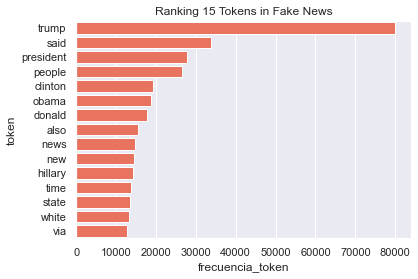
\includegraphics{output_63_0.png}
\caption{Ranking 15 Tokens in Fake News}
\end{figure}

\begin{Shaded}
\begin{Highlighting}[]
\NormalTok{p2 }\OperatorTok{=}\NormalTok{ sns.barplot(data}\OperatorTok{=}\NormalTok{df\_no\_fake\_sort\_not\_StopWords.head(}\DecValTok{15}\NormalTok{), x}\OperatorTok{=}\StringTok{\textquotesingle{}frecuencia\_token\textquotesingle{}}\NormalTok{, y}\OperatorTok{=}\StringTok{\textquotesingle{}token\textquotesingle{}}\NormalTok{, color}\OperatorTok{=}\StringTok{\textquotesingle{}cyan\textquotesingle{}}\NormalTok{).}\BuiltInTok{set}\NormalTok{(title}\OperatorTok{=}\StringTok{\textquotesingle{}Ranking 15 Tokens in Not Fake News\textquotesingle{}}\NormalTok{) }
\end{Highlighting}
\end{Shaded}

\begin{figure}
\centering
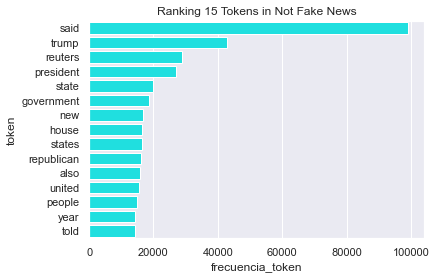
\includegraphics{output_64_0.png}
\caption{Ranking 15 Tokens in Not Fake News}
\end{figure}

\hypertarget{odds-ratio}{%
\subsection{Odds Ratio}\label{odds-ratio}}

A continuación, se estudia qué palabras se utilizan de forma más
diferenciada en cada tipo de noticia (fake / no fake), es decir,
palabras que utiliza mucho en las fake news y que no se utilizan tanto
en las no fakes, y viceversa.

Una forma de hacer este análisis es mediante el odds ratio de las
frecuencias.

Sea \(\hspace{0.2cm}p_k1 = \cfrac{n_{k1} + 1}{N_1 + 1}\hspace{0.2cm}\) y
\(\hspace{0.2cm}p_k0 = \cfrac{n_{k0} + 1}{N_0 +1}\)

\[OR(Fake|NoFake , k) = \dfrac{ p_{k1} }{ p_{k0} }\]

Donde:

\(n_{k1}\) el número de veces que aparece el token \(k\) en las
\textbf{fake news}.

\(n_{k0}\) el numero de veces que aparece el termino \(k\) en las
\textbf{no fake news}.

\(N_1\) es el número de tokens, contando repeticiones, que aparecen en
las \textbf{fake news}.

\(N_0\) es el número de tokens, contando repeticiones, que aparecen en
las \textbf{no fake news}

Por tanto:

\(p_{k1} \approx\) proporcion de apariciones del token \(k\) en las
\textbf{fake news}

\(p_{k0} \approx\) proporcion de apariciones del token \(k\) en las
\textbf{no fake news}

Si \(OddsRatio(k) = \dfrac{ p_k1 }{ p_k0 } = h\) , entonces:

Si \(h>1\) \(\Rightarrow\) el token \(k\) es \(h\) veces mas frecuente
en las \textbf{fake news} que en las \textbf{no fake news}, ya que
\(p_{k1} = h \cdot p_{k0}\)

Si \(h \in (0 , 1)\) \(\Rightarrow\) el token \(k\) es \(1/h\) veces mas
frecuente en las \textbf{no fake news} que en las \textbf{fake news}, ya
que \(p_{k0} = (1/h) \cdot p_{k1}\) , donde \((1/h)>1\)

Si \(h= 1\) \(\Rightarrow\) el token \(k\) es igual de frecuente en las
\textbf{fake news} que en las \textbf{no fake news}, ya que
\(p_{k1} = p_{k0}\)

A continuacion definimos funciones para calcular \(n_{k1}\) y \(n_{k0}\)
en \texttt{Python}

\begin{Shaded}
\begin{Highlighting}[]
\KeywordTok{def}\NormalTok{ n\_k1(token) : }

\NormalTok{    n\_k1 }\OperatorTok{=}\NormalTok{ df\_fake\_sort\_not\_StopWords.loc[ df\_fake\_sort\_not\_StopWords[}\StringTok{\textquotesingle{}token\textquotesingle{}}\NormalTok{]}\OperatorTok{==}\NormalTok{token , }\StringTok{\textquotesingle{}frecuencia\_token\textquotesingle{}}\NormalTok{]}

    \ControlFlowTok{return}\NormalTok{(n\_k1)}
\end{Highlighting}
\end{Shaded}

\begin{Shaded}
\begin{Highlighting}[]
\KeywordTok{def}\NormalTok{ n\_k0(token) : }

\NormalTok{    n\_k0 }\OperatorTok{=}\NormalTok{ df\_no\_fake\_sort\_not\_StopWords.loc[ df\_no\_fake\_sort\_not\_StopWords[}\StringTok{\textquotesingle{}token\textquotesingle{}}\NormalTok{]}\OperatorTok{==}\NormalTok{token , }\StringTok{\textquotesingle{}frecuencia\_token\textquotesingle{}}\NormalTok{]}

    \ControlFlowTok{return}\NormalTok{(n\_k0)}
\end{Highlighting}
\end{Shaded}

Probamos las funciones para algunos tokens concretos:

\begin{Shaded}
\begin{Highlighting}[]
\NormalTok{n\_k0(}\StringTok{\textquotesingle{}trump\textquotesingle{}}\NormalTok{) }
\end{Highlighting}
\end{Shaded}

\begin{verbatim}
17    42755
Name: frecuencia_token 
\end{verbatim}

\begin{Shaded}
\begin{Highlighting}[]
\NormalTok{n\_k1(}\StringTok{\textquotesingle{}trump\textquotesingle{}}\NormalTok{) }
\end{Highlighting}
\end{Shaded}

\begin{verbatim}
10    79922
Name: frecuencia_token 
\end{verbatim}

Estas salidas nos indican que el nº de veces que aparece el token
`trump' en el conjunto de las fake news es 79922 , mientras que en el
conjunto de las no fake news es 42755.

\(N_0\) y \(N_1\) coinciden con el nº de tokens, contando repeticiones y
sin considerar las stopwords, que aparecen el las no fake y fake news,
respectivamente:

\begin{Shaded}
\begin{Highlighting}[]
\NormalTok{Fake\_News\_Tokens\_not\_StopWords }\OperatorTok{=}\NormalTok{ Fake\_News\_Tokens[ }\OperatorTok{\textasciitilde{}}\NormalTok{ Fake\_News\_Tokens[}\StringTok{\textquotesingle{}token\textquotesingle{}}\NormalTok{].isin(stop\_words) ]}

\NormalTok{Fake\_News\_Tokens\_not\_StopWords}
\end{Highlighting}
\end{Shaded}

\begin{verbatim}
       id_text       token Fake
       
0            0      donald    1
0            0       trump    1
0            0        wish    1
0            0   americans    1
0            0       happy    1

...        ...         ...  ...

44897    44897      energy    0
44897    44897  technology    0
44897    44897    aviation    0
44897    44897       among    0
44897    44897      others    0
\end{verbatim}

\begin{Shaded}
\begin{Highlighting}[]
\NormalTok{Fake\_News\_Tokens\_not\_StopWords.groupby(by}\OperatorTok{=}\StringTok{\textquotesingle{}Fake\textquotesingle{}}\NormalTok{)[}\StringTok{\textquotesingle{}token\textquotesingle{}}\NormalTok{].count()}
\end{Highlighting}
\end{Shaded}

\begin{verbatim}
Fake
0    4782198
1    5396339

Name: token
\end{verbatim}

\begin{Shaded}
\begin{Highlighting}[]
\NormalTok{N0 }\OperatorTok{=}\NormalTok{ Fake\_News\_Tokens\_not\_StopWords.groupby(by}\OperatorTok{=}\StringTok{\textquotesingle{}Fake\textquotesingle{}}\NormalTok{)[}\StringTok{\textquotesingle{}token\textquotesingle{}}\NormalTok{].count()[}\DecValTok{0}\NormalTok{]}

\NormalTok{N1 }\OperatorTok{=}\NormalTok{ Fake\_News\_Tokens\_not\_StopWords.groupby(by}\OperatorTok{=}\StringTok{\textquotesingle{}Fake\textquotesingle{}}\NormalTok{)[}\StringTok{\textquotesingle{}token\textquotesingle{}}\NormalTok{].count()[}\DecValTok{1}\NormalTok{]}
\end{Highlighting}
\end{Shaded}

\begin{Shaded}
\begin{Highlighting}[]
\NormalTok{N0}
\end{Highlighting}
\end{Shaded}

\begin{verbatim}
4782198
\end{verbatim}

\begin{Shaded}
\begin{Highlighting}[]
\NormalTok{N1}
\end{Highlighting}
\end{Shaded}

\begin{verbatim}
5396339
\end{verbatim}

Como ejemplo vamos a calcular el Odds Ratio fake - no fake para el toke
`trump' :

\begin{Shaded}
\begin{Highlighting}[]
\NormalTok{n\_k0(}\StringTok{\textquotesingle{}trump\textquotesingle{}}\NormalTok{) }\OperatorTok{/}\NormalTok{ N0 }
\end{Highlighting}
\end{Shaded}

\begin{verbatim}
17    0.00894
Name: frecuencia_token, dtype: float64
\end{verbatim}

\begin{Shaded}
\begin{Highlighting}[]
\NormalTok{n\_k1(}\StringTok{\textquotesingle{}trump\textquotesingle{}}\NormalTok{) }\OperatorTok{/}\NormalTok{ N1}
\end{Highlighting}
\end{Shaded}

\begin{verbatim}
10    0.01481
Name: frecuencia_token, dtype: float64
\end{verbatim}

\begin{Shaded}
\begin{Highlighting}[]
\CommentTok{\# Odds Ratio fake {-} no fake para el token \textquotesingle{}trump\textquotesingle{}}

\BuiltInTok{float}\NormalTok{( n\_k0(}\StringTok{\textquotesingle{}trump\textquotesingle{}}\NormalTok{) }\OperatorTok{/}\NormalTok{ N0 ) }\OperatorTok{/} \BuiltInTok{float}\NormalTok{( n\_k1(}\StringTok{\textquotesingle{}trump\textquotesingle{}}\NormalTok{) }\OperatorTok{/}\NormalTok{ N1 )}
\end{Highlighting}
\end{Shaded}

\begin{verbatim}
1.6565622548396417
\end{verbatim}

Por tanto el token `trump' es 1.66 veces mas frecuente en las fake news
que en las no fake.

\begin{Shaded}
\begin{Highlighting}[]
\NormalTok{df1 }\OperatorTok{=}\NormalTok{ df\_fake\_sort\_not\_StopWords.sort\_values(by}\OperatorTok{=}\NormalTok{[}\StringTok{"token"}\NormalTok{]).reset\_index(drop}\OperatorTok{=}\VariableTok{True}\NormalTok{)}
\NormalTok{df1}
\end{Highlighting}
\end{Shaded}

\begin{verbatim}
         index  Fake       token  frecuencia_token
0       125805     1          aa                24
1       125806     1         aaa                 9
2       125807     1  aaaaaaaand                 1
3       125808     1   aaaaackkk                 1
4       125809     1  aaaaapkfhk                 1
...        ...   ...         ...               ...
125561  251605     1        ””it                 0
125562  251606     1      ””when                 0
125563  251607     1         •if                 0
125564  251608     1    $emoji1$                 0
125565  251609     1    $emoji2$️                 0
\end{verbatim}

\begin{Shaded}
\begin{Highlighting}[]
\NormalTok{df0 }\OperatorTok{=}\NormalTok{ df\_no\_fake\_sort\_not\_StopWords.sort\_values(by}\OperatorTok{=}\NormalTok{[}\StringTok{"token"}\NormalTok{]).reset\_index(drop}\OperatorTok{=}\VariableTok{True}\NormalTok{)}
\NormalTok{df0}
\end{Highlighting}
\end{Shaded}

\begin{verbatim}
         index  Fake       token  frecuencia_token
0            0     0          aa                22
1            1     0         aaa                 7
2            2     0  aaaaaaaand                 0
3            3     0   aaaaackkk                 0
4            4     0  aaaaapkfhk                 0
...        ...   ...         ...               ...
125561  125800     0        ””it                 1
125562  125801     0      ””when                 1
125563  125802     0         •if                 3
125564  125803     0    $emoji1$                 3
125565  125804     0    ️$emoji2$                 1
\end{verbatim}

\begin{Shaded}
\begin{Highlighting}[]

\NormalTok{n\_k0\_vector }\OperatorTok{=}\NormalTok{ df0[}\StringTok{\textquotesingle{}frecuencia\_token\textquotesingle{}}\NormalTok{]}

\NormalTok{n\_k1\_vector }\OperatorTok{=}\NormalTok{ df1[}\StringTok{\textquotesingle{}frecuencia\_token\textquotesingle{}}\NormalTok{]}


\NormalTok{Odds\_ratio }\OperatorTok{=}\NormalTok{ ( ( n\_k1\_vector }\OperatorTok{+} \DecValTok{1}\NormalTok{ ) }\OperatorTok{/}\NormalTok{ ( N1 }\OperatorTok{+} \DecValTok{1}\NormalTok{) ) }\OperatorTok{/}\NormalTok{ ( ( n\_k0\_vector }\OperatorTok{+} \DecValTok{1}\NormalTok{ ) }\OperatorTok{/}\NormalTok{ ( N0 }\OperatorTok{+} \DecValTok{1}\NormalTok{) )}
\end{Highlighting}
\end{Shaded}

\begin{Shaded}
\begin{Highlighting}[]
\NormalTok{df0[}\StringTok{\textquotesingle{}Odds\_ratio\_Fake\_NotFake\textquotesingle{}}\NormalTok{] }\OperatorTok{=}\NormalTok{ Odds\_ratio  }
\NormalTok{df1[}\StringTok{\textquotesingle{}Odds\_ratio\_Fake\_NotFake\textquotesingle{}}\NormalTok{] }\OperatorTok{=}\NormalTok{ Odds\_ratio  }

\NormalTok{df0[}\StringTok{\textquotesingle{}Odds\_ratio\_NotFake\_Fake\textquotesingle{}}\NormalTok{] }\OperatorTok{=} \DecValTok{1} \OperatorTok{/}\NormalTok{ df0[}\StringTok{"Odds\_ratio\_Fake\_NotFake"}\NormalTok{] }
\NormalTok{df1[}\StringTok{\textquotesingle{}Odds\_ratio\_NotFake\_Fake\textquotesingle{}}\NormalTok{] }\OperatorTok{=} \DecValTok{1} \OperatorTok{/}\NormalTok{ df1[}\StringTok{"Odds\_ratio\_Fake\_NotFake"}\NormalTok{]  }
\end{Highlighting}
\end{Shaded}

\begin{Shaded}
\begin{Highlighting}[]
\NormalTok{df0}
\end{Highlighting}
\end{Shaded}

\begin{verbatim}
         index  Fake       token  frecuencia_token  Odds_ratio_Fake_NotFake  \
0            0     0          aa                22                 0.963253   
1            1     0         aaa                 7                 1.107741   
2            2     0  aaaaaaaand                 0                 1.772386   
3            3     0   aaaaackkk                 0                 1.772386   
4            4     0  aaaaapkfhk                 0                 1.772386   
...        ...   ...         ...               ...                      ...   
125561  125800     0        ””it                 1                 0.443097   
125562  125801     0      ””when                 1                 0.443097   
125563  125802     0         •if                 3                 0.221548   
125564  125803     0    ️$emoji1$                 3                 0.221548   
125565  125804     0    $emoji2$                 1                 0.443097   

        Odds_ratio_NotFake_Fake  
0                      1.038149  
1                      0.902738  
2                      0.564211  
3                      0.564211  
4                      0.564211  
...                         ...  
125561                 2.256845  
125562                 2.256845  
125563                 4.513689  
125564                 4.513689  
125565                 2.256845  
\end{verbatim}

\begin{Shaded}
\begin{Highlighting}[]
\NormalTok{df1}
\end{Highlighting}
\end{Shaded}

\begin{Shaded}
\begin{Highlighting}[]
\NormalTok{df0.sort\_values(by}\OperatorTok{=}\NormalTok{[}\StringTok{"Odds\_ratio\_Fake\_NotFake"}\NormalTok{], ascending}\OperatorTok{=}\VariableTok{False}\NormalTok{).reset\_index(drop}\OperatorTok{=}\VariableTok{True}\NormalTok{).head(}\DecValTok{5}\NormalTok{)}
\end{Highlighting}
\end{Shaded}

\begin{verbatim}
    index  Fake            token  frecuencia_token  Odds_ratio_Fake_NotFake  \
0   35830     0          finicum                 0               320.801884   
1  114264     0        wikimedia                 0               200.279629   
2  109040     0  uninterruptible                 0               189.645313   
3   78372     0     philosophers                 0               186.100540   
4   60711     0          lovable                 0               183.441961   

   Odds_ratio_NotFake_Fake  
0                 0.003117  
1                 0.004993  
2                 0.005273  
3                 0.005373  
4                 0.005451
\end{verbatim}

\begin{Shaded}
\begin{Highlighting}[]
\NormalTok{df0.sort\_values(by}\OperatorTok{=}\NormalTok{[}\StringTok{"Odds\_ratio\_NotFake\_Fake"}\NormalTok{], ascending}\OperatorTok{=}\VariableTok{False}\NormalTok{).reset\_index(drop}\OperatorTok{=}\VariableTok{True}\NormalTok{).head(}\DecValTok{5}\NormalTok{)}
\end{Highlighting}
\end{Shaded}

\begin{verbatim}
    index  Fake      token  frecuencia_token  Odds_ratio_Fake_NotFake  \
0  106864     0    trump’s             11629                 0.000076   
1   72989     0    obama’s              2132                 0.000415   
2   18791     0  clinton’s              1604                 0.000552   
3   76630     0    party’s              1101                 0.000804   
4   98675     0    state’s              1010                 0.000877   

   Odds_ratio_NotFake_Fake  
0             13123.551362  
1              2406.924768  
2              1811.117793  
3              1243.521376  
4              1140.834946
\end{verbatim}

\begin{Shaded}
\begin{Highlighting}[]
\NormalTok{df1.sort\_values(by}\OperatorTok{=}\NormalTok{[}\StringTok{"Odds\_ratio\_Fake\_NotFake"}\NormalTok{], ascending}\OperatorTok{=}\VariableTok{False}\NormalTok{).reset\_index(drop}\OperatorTok{=}\VariableTok{True}\NormalTok{).head(}\DecValTok{5}\NormalTok{)}
\end{Highlighting}
\end{Shaded}

\begin{verbatim}
    index  Fake            token  frecuencia_token  Odds_ratio_Fake_NotFake  \
0  161635     1          finicum               361               320.801884   
1  240069     1        wikimedia               225               200.279629   
2  234845     1  uninterruptible               213               189.645313   
3  204177     1     philosophers               209               186.100540   
4  186516     1          lovable               206               183.441961   

   Odds_ratio_NotFake_Fake  
0                 0.003117  
1                 0.004993  
2                 0.005273  
3                 0.005373  
4                 0.005451
\end{verbatim}

\begin{Shaded}
\begin{Highlighting}[]
\NormalTok{df1.sort\_values(by}\OperatorTok{=}\NormalTok{[}\StringTok{"Odds\_ratio\_NotFake\_Fake"}\NormalTok{], ascending}\OperatorTok{=}\VariableTok{False}\NormalTok{).reset\_index(drop}\OperatorTok{=}\VariableTok{True}\NormalTok{).head(}\DecValTok{5}\NormalTok{)}
\end{Highlighting}
\end{Shaded}

\begin{verbatim}
    index  Fake      token  frecuencia_token  Odds_ratio_Fake_NotFake  \
0  232669     1    trump’s                 0                 0.000076   
1  198794     1    obama’s                 0                 0.000415   
2  144596     1  clinton’s                 0                 0.000552   
3  202435     1    party’s                 0                 0.000804   
4  224480     1    state’s                 0                 0.000877   

   Odds_ratio_NotFake_Fake  
0             13123.551362  
1              2406.924768  
2              1811.117793  
3              1243.521376  
4              1140.834946 
\end{verbatim}

Notese que en ambos data sets las columnas Odds\_ratio\_Fake\_NotFake y
Odds\_ratio\_NotFake\_Fake son las mismas, por tanto podemos construir
un nuevo data set solo con esas columnas y otra para los tokens, a
partir de cualquiera de esos dos data-sets.

\begin{Shaded}
\begin{Highlighting}[]
\NormalTok{Odds\_ratio\_df }\OperatorTok{=}\NormalTok{ df1.loc[: , [}\StringTok{\textquotesingle{}token\textquotesingle{}}\NormalTok{, }\StringTok{\textquotesingle{}Odds\_ratio\_Fake\_NotFake\textquotesingle{}}\NormalTok{ , }\StringTok{\textquotesingle{}Odds\_ratio\_NotFake\_Fake\textquotesingle{}}\NormalTok{]]  }

\NormalTok{Odds\_ratio\_df}
\end{Highlighting}
\end{Shaded}

\begin{Shaded}
\begin{Highlighting}[]
\NormalTok{Odds\_ratio\_df.sort\_values(by}\OperatorTok{=}\NormalTok{[}\StringTok{"Odds\_ratio\_Fake\_NotFake"}\NormalTok{], ascending}\OperatorTok{=}\VariableTok{False}\NormalTok{).head(}\DecValTok{15}\NormalTok{)}
\end{Highlighting}
\end{Shaded}

\begin{verbatim}
                  token  Odds_ratio_Fake_NotFake  Odds_ratio_NotFake_Fake
35775           finicum               320.801884                 0.003117
114071        wikimedia               200.279629                 0.004993
108870  uninterruptible               189.645313                 0.005273
78242      philosophers               186.100540                 0.005373
60612           lovable               183.441961                 0.005451
91113           savants               182.555768                 0.005478
67583         moralists               182.555768                 0.005478
97785             spore               182.555768                 0.005478
84324           rascals               181.669575                 0.005504
32976       evangelists               181.669575                 0.005504
63302        masochists               181.669575                 0.005504
11482            boiler               172.586096                 0.005794
13727             bundy               170.813710                 0.005854
92025        screengrab               167.490486                 0.005970
113747           whined               166.604293                 0.006002
\end{verbatim}

\begin{Shaded}
\begin{Highlighting}[]
\NormalTok{Odds\_ratio\_df.sort\_values(by}\OperatorTok{=}\NormalTok{[}\StringTok{"Odds\_ratio\_NotFake\_Fake"}\NormalTok{], ascending}\OperatorTok{=}\VariableTok{False}\NormalTok{).head(}\DecValTok{15}\NormalTok{)}
\end{Highlighting}
\end{Shaded}

\begin{verbatim}
                   token  Odds_ratio_Fake_NotFake  Odds_ratio_NotFake_Fake
106696           trump’s                 0.000076             13123.551362
72874            obama’s                 0.000415              2406.924768
18756          clinton’s                 0.000552              1811.117793
76500            party’s                 0.000804              1243.521376
98529            state’s                 0.000877              1140.834946
80975        president’s                 0.000979              1021.222183
83999            rakhine                 0.000987              1013.323226
1242    administration’s                 0.001157               864.371483
88673           rohingya                 0.001294               772.969276
117944              zuma                 0.001298               770.712432
82344         puigdemont                 0.001372               728.960807
17524            china’s                 0.001400               714.291317
89715           russia’s                 0.001439               695.108137
21888          country’s                 0.001541               648.842823
69047            myanmar                 0.001579               633.496280
\end{verbatim}

\begin{Shaded}
\begin{Highlighting}[]

\NormalTok{p1 }\OperatorTok{=}\NormalTok{ sns.barplot(data}\OperatorTok{=}\NormalTok{Odds\_ratio\_df.sort\_values(by}\OperatorTok{=}\NormalTok{[}\StringTok{"Odds\_ratio\_Fake\_NotFake"}\NormalTok{], ascending}\OperatorTok{=}\VariableTok{False}\NormalTok{).head(}\DecValTok{15}\NormalTok{) ,}
\NormalTok{                 x}\OperatorTok{=}\StringTok{\textquotesingle{}Odds\_ratio\_Fake\_NotFake\textquotesingle{}}\NormalTok{, y}\OperatorTok{=}\StringTok{\textquotesingle{}token\textquotesingle{}}\NormalTok{, color}\OperatorTok{=}\StringTok{\textquotesingle{}tomato\textquotesingle{}}\NormalTok{).}\BuiltInTok{set}\NormalTok{(title}\OperatorTok{=}\StringTok{\textquotesingle{}Ranking 15 most representative tokens in Fake News\textquotesingle{}}\NormalTok{) }
\end{Highlighting}
\end{Shaded}

\begin{figure}
\centering
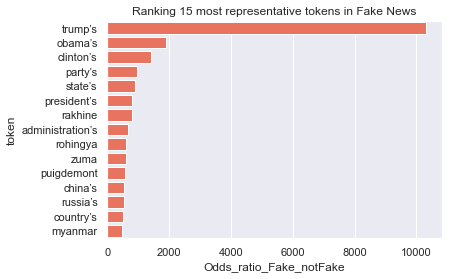
\includegraphics{output_95_0.png}
\caption{png}
\end{figure}

\begin{Shaded}
\begin{Highlighting}[]
\NormalTok{p2 }\OperatorTok{=}\NormalTok{ sns.barplot(data}\OperatorTok{=}\NormalTok{Odds\_ratio\_df.sort\_values(by}\OperatorTok{=}\NormalTok{[}\StringTok{"Odds\_ratio\_NotFake\_Fake"}\NormalTok{], ascending}\OperatorTok{=}\VariableTok{False}\NormalTok{).head(}\DecValTok{15}\NormalTok{) ,}
\NormalTok{                 x}\OperatorTok{=}\StringTok{\textquotesingle{}Odds\_ratio\_NotFake\_Fake\textquotesingle{}}\NormalTok{, y}\OperatorTok{=}\StringTok{\textquotesingle{}token\textquotesingle{}}\NormalTok{, color}\OperatorTok{=}\StringTok{\textquotesingle{}cyan\textquotesingle{}}\NormalTok{).}\BuiltInTok{set}\NormalTok{(title}\OperatorTok{=}\StringTok{\textquotesingle{}Ranking 15 most representative tokens in Not Fake News\textquotesingle{}}\NormalTok{) }
\end{Highlighting}
\end{Shaded}

\begin{figure}
\centering
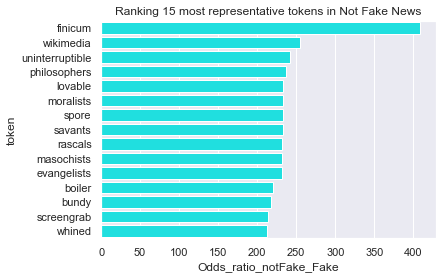
\includegraphics{output_96_0.png}
\caption{png}
\end{figure}

\end{document}
